% \newpage
% % \newcommand{\type}{router}
% % \newcommand{\status}{stable}


% Um einen WLAN-Router als Freifunk Router zu nutzen ist es erforderlich, das Freifunk Betriebssystem – die Freifunk Firmware – zu installieren. Die Installation ist sehr einfach und du benötigst keine technischen Kenntnisse. Wenn du dieser Anleitung folgst kann eigentlich nichts schiefgehen.\\

% {\Large 1. Firmware herunterladen} \\

% \newpage
\columnseprule2pt 
\columnsep7mm
\def\columnseprulecolor{\color{FFmagenta}}
% {
% % \setlength{\columnseprule}{3pt}
% % \setlength{\columnsep}{5pt}
% % \def\columnseprulecolor{\color{FFmagenta}}

% \begin{multicols}{2}
% [
% \section{First Section}
% All human things are subject to decay. And when fate summons, Monarchs must obey.
% ]
% asdsadasdads
 
% % \begin{wrapfigure}{l}{0.5\linewidth}
% 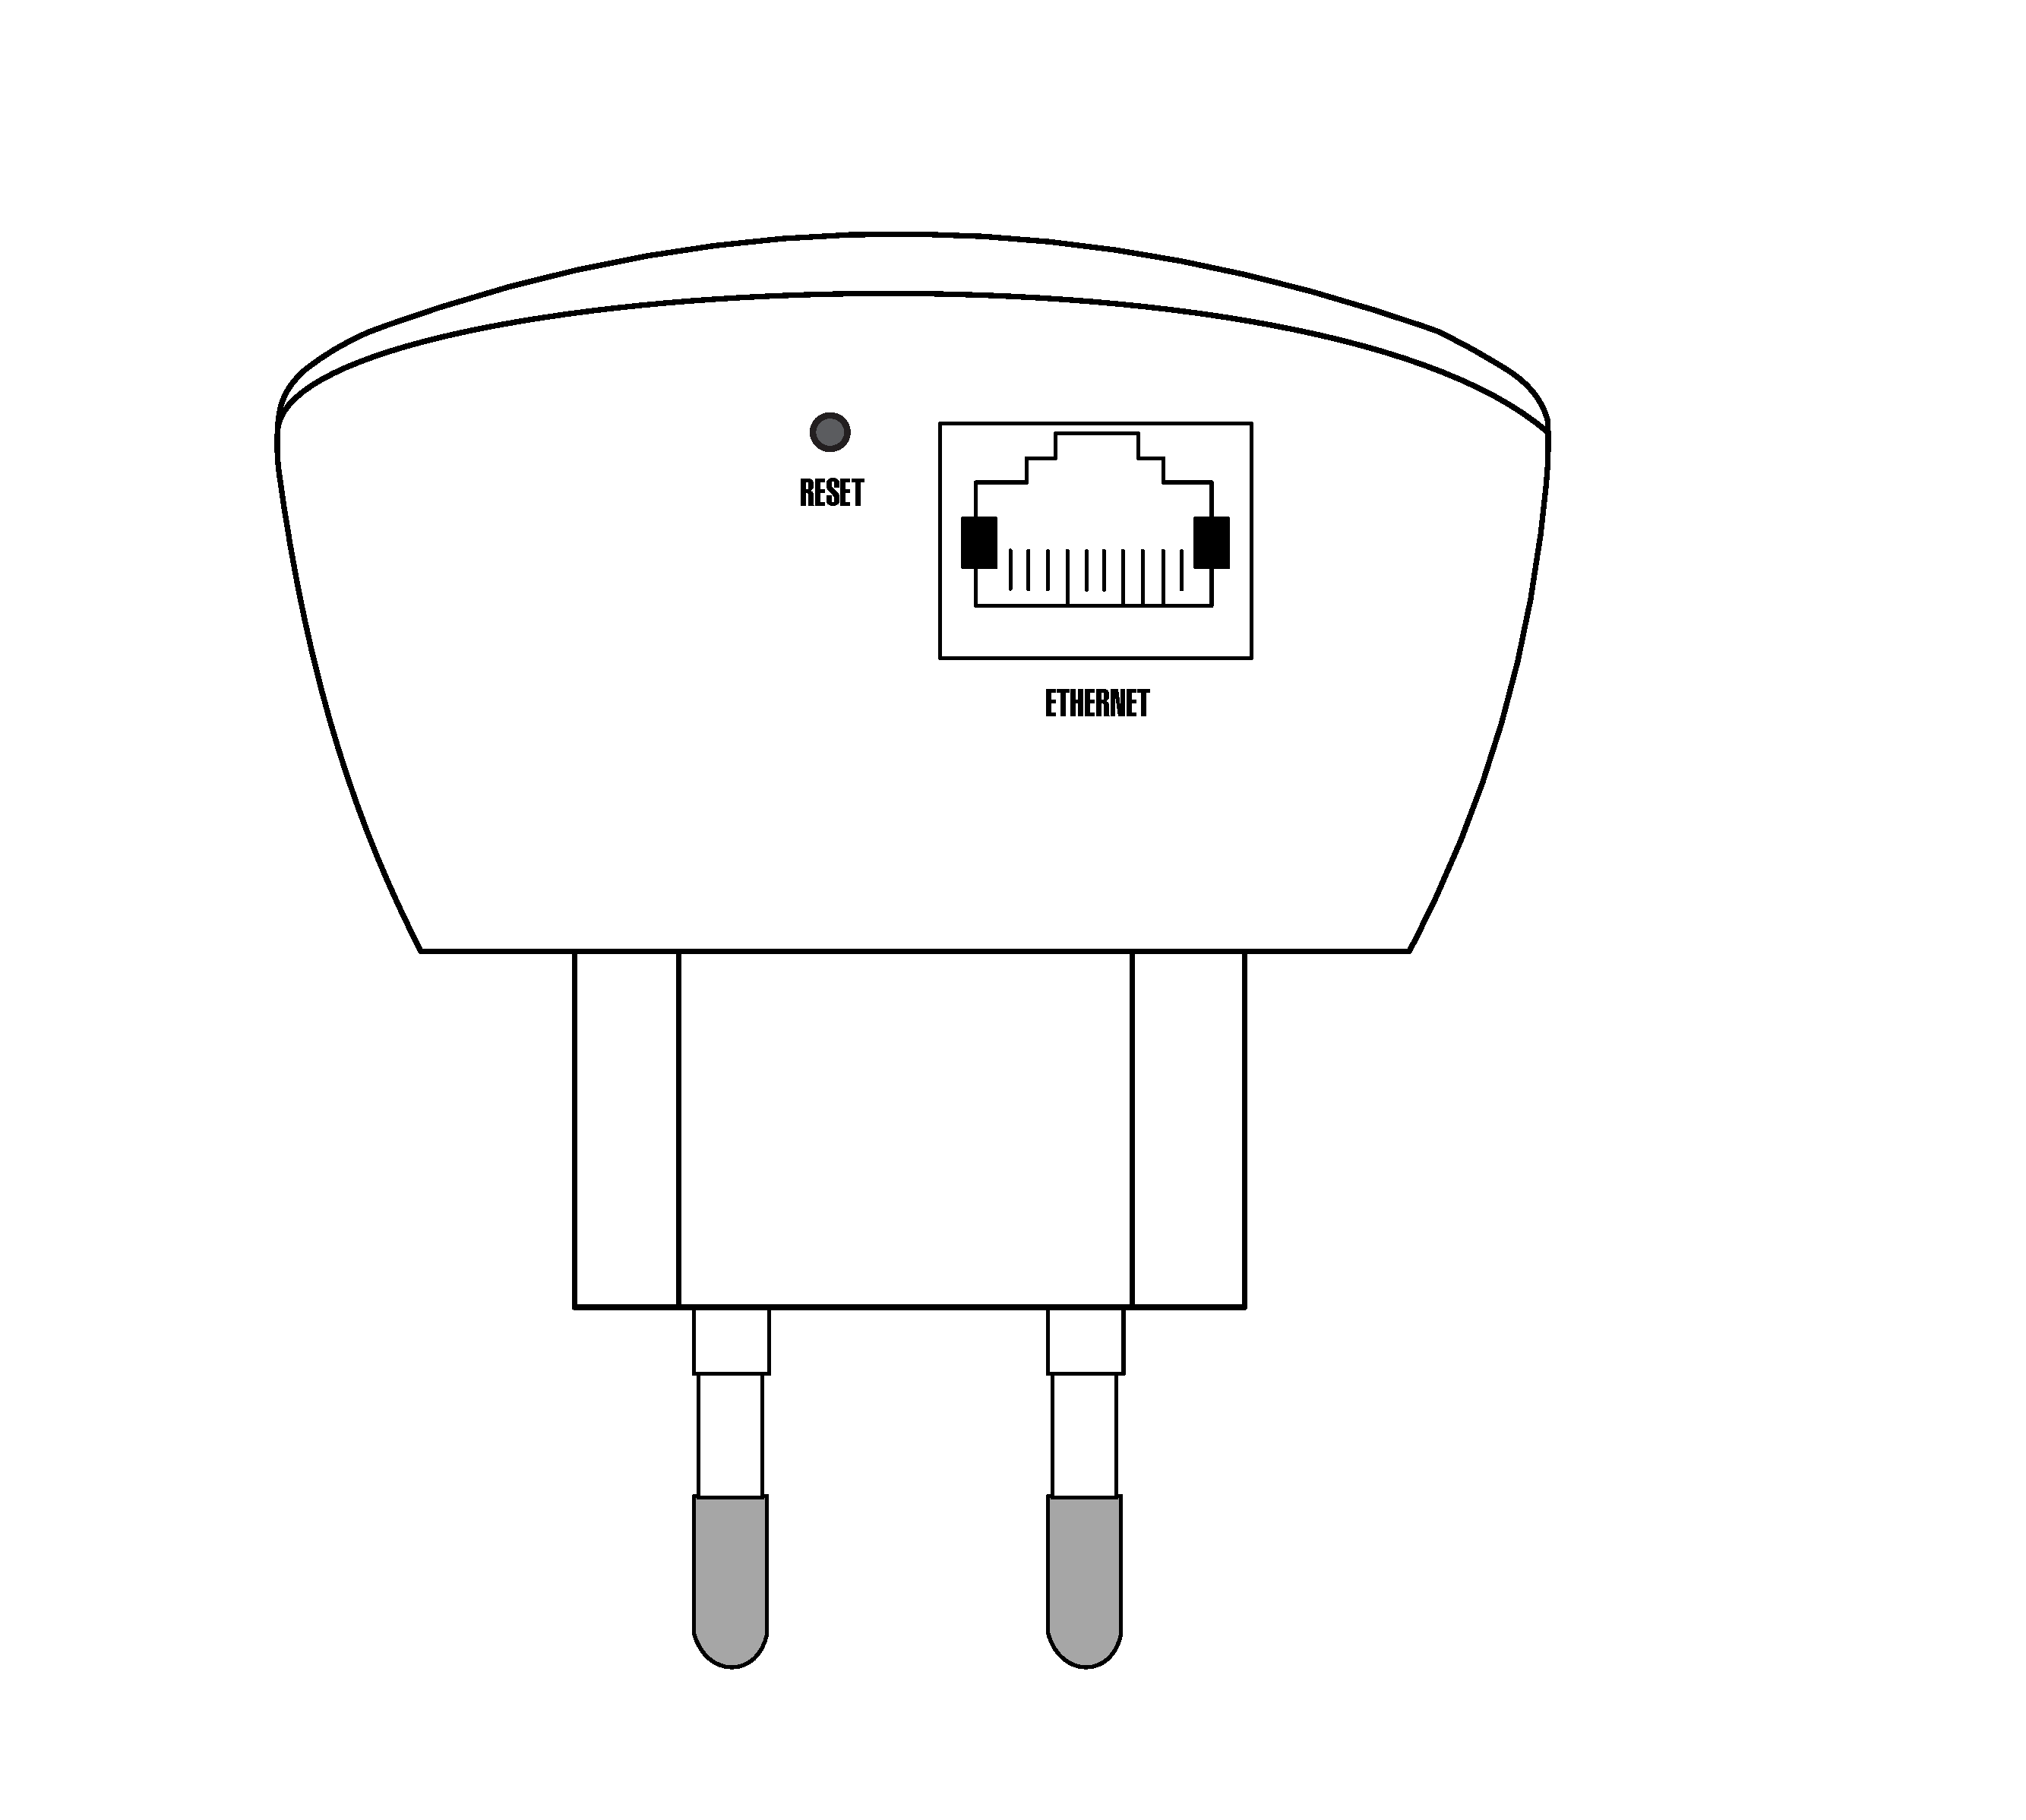
\includegraphics[width=\linewidth*0.3]{./back.pdf}}
% % \caption{This is the Share\LaTeX{} logo}
% % \end{wrapfigure}
 
% \columnbreak
 
% This will be in a new column, here is some text without a meaning.  This text 
% should show what a printed text will look like at this place.
 
% If you read this text, you will get no information.  Really?  Is there 
% no information?  Is there...
% \end{multicols}
% }

% \begin{multicols}{2}[\section*{Den Router Anschließen}]
% \vspace{-1cm}
% \textcolor{FFmagenta}{\rule[1cm]{0.5\textwidth}{0.75mm}}
% % \begin{figure}[h]
% % \makebox[width=0.5\textwidth]{ 
% 	% 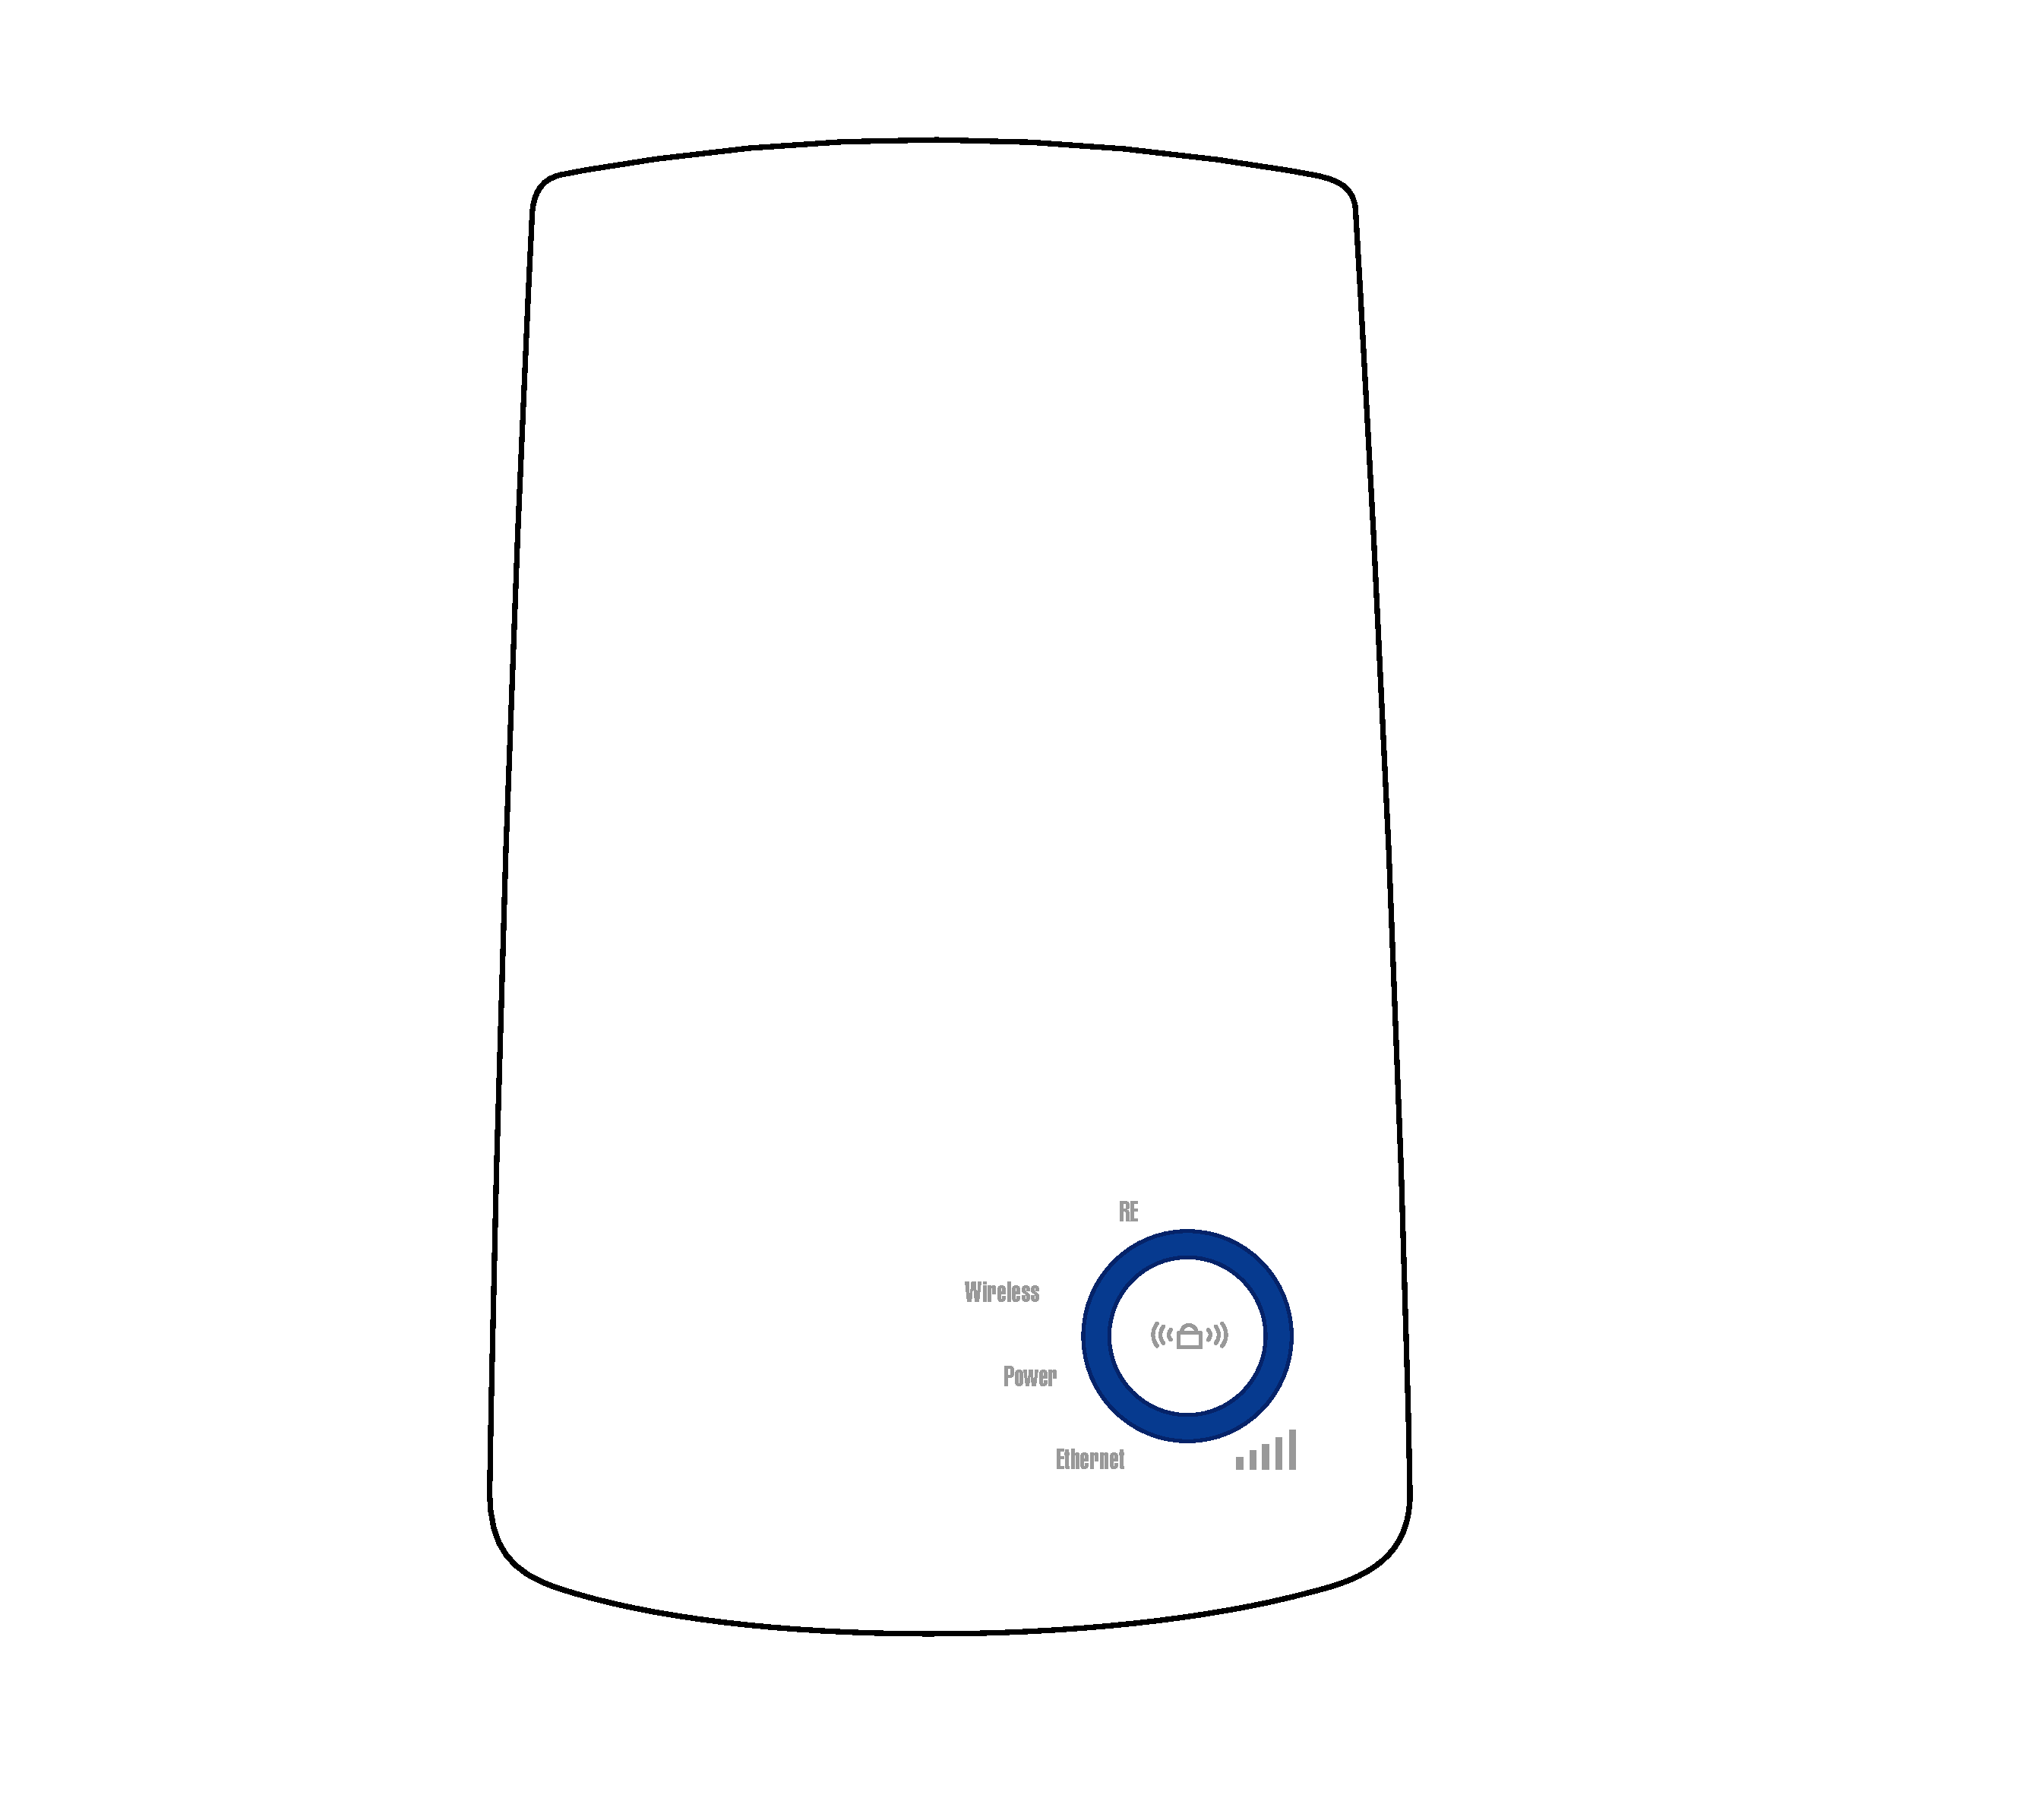
\includegraphics[scale=0.25]{./front.pdf}
% 	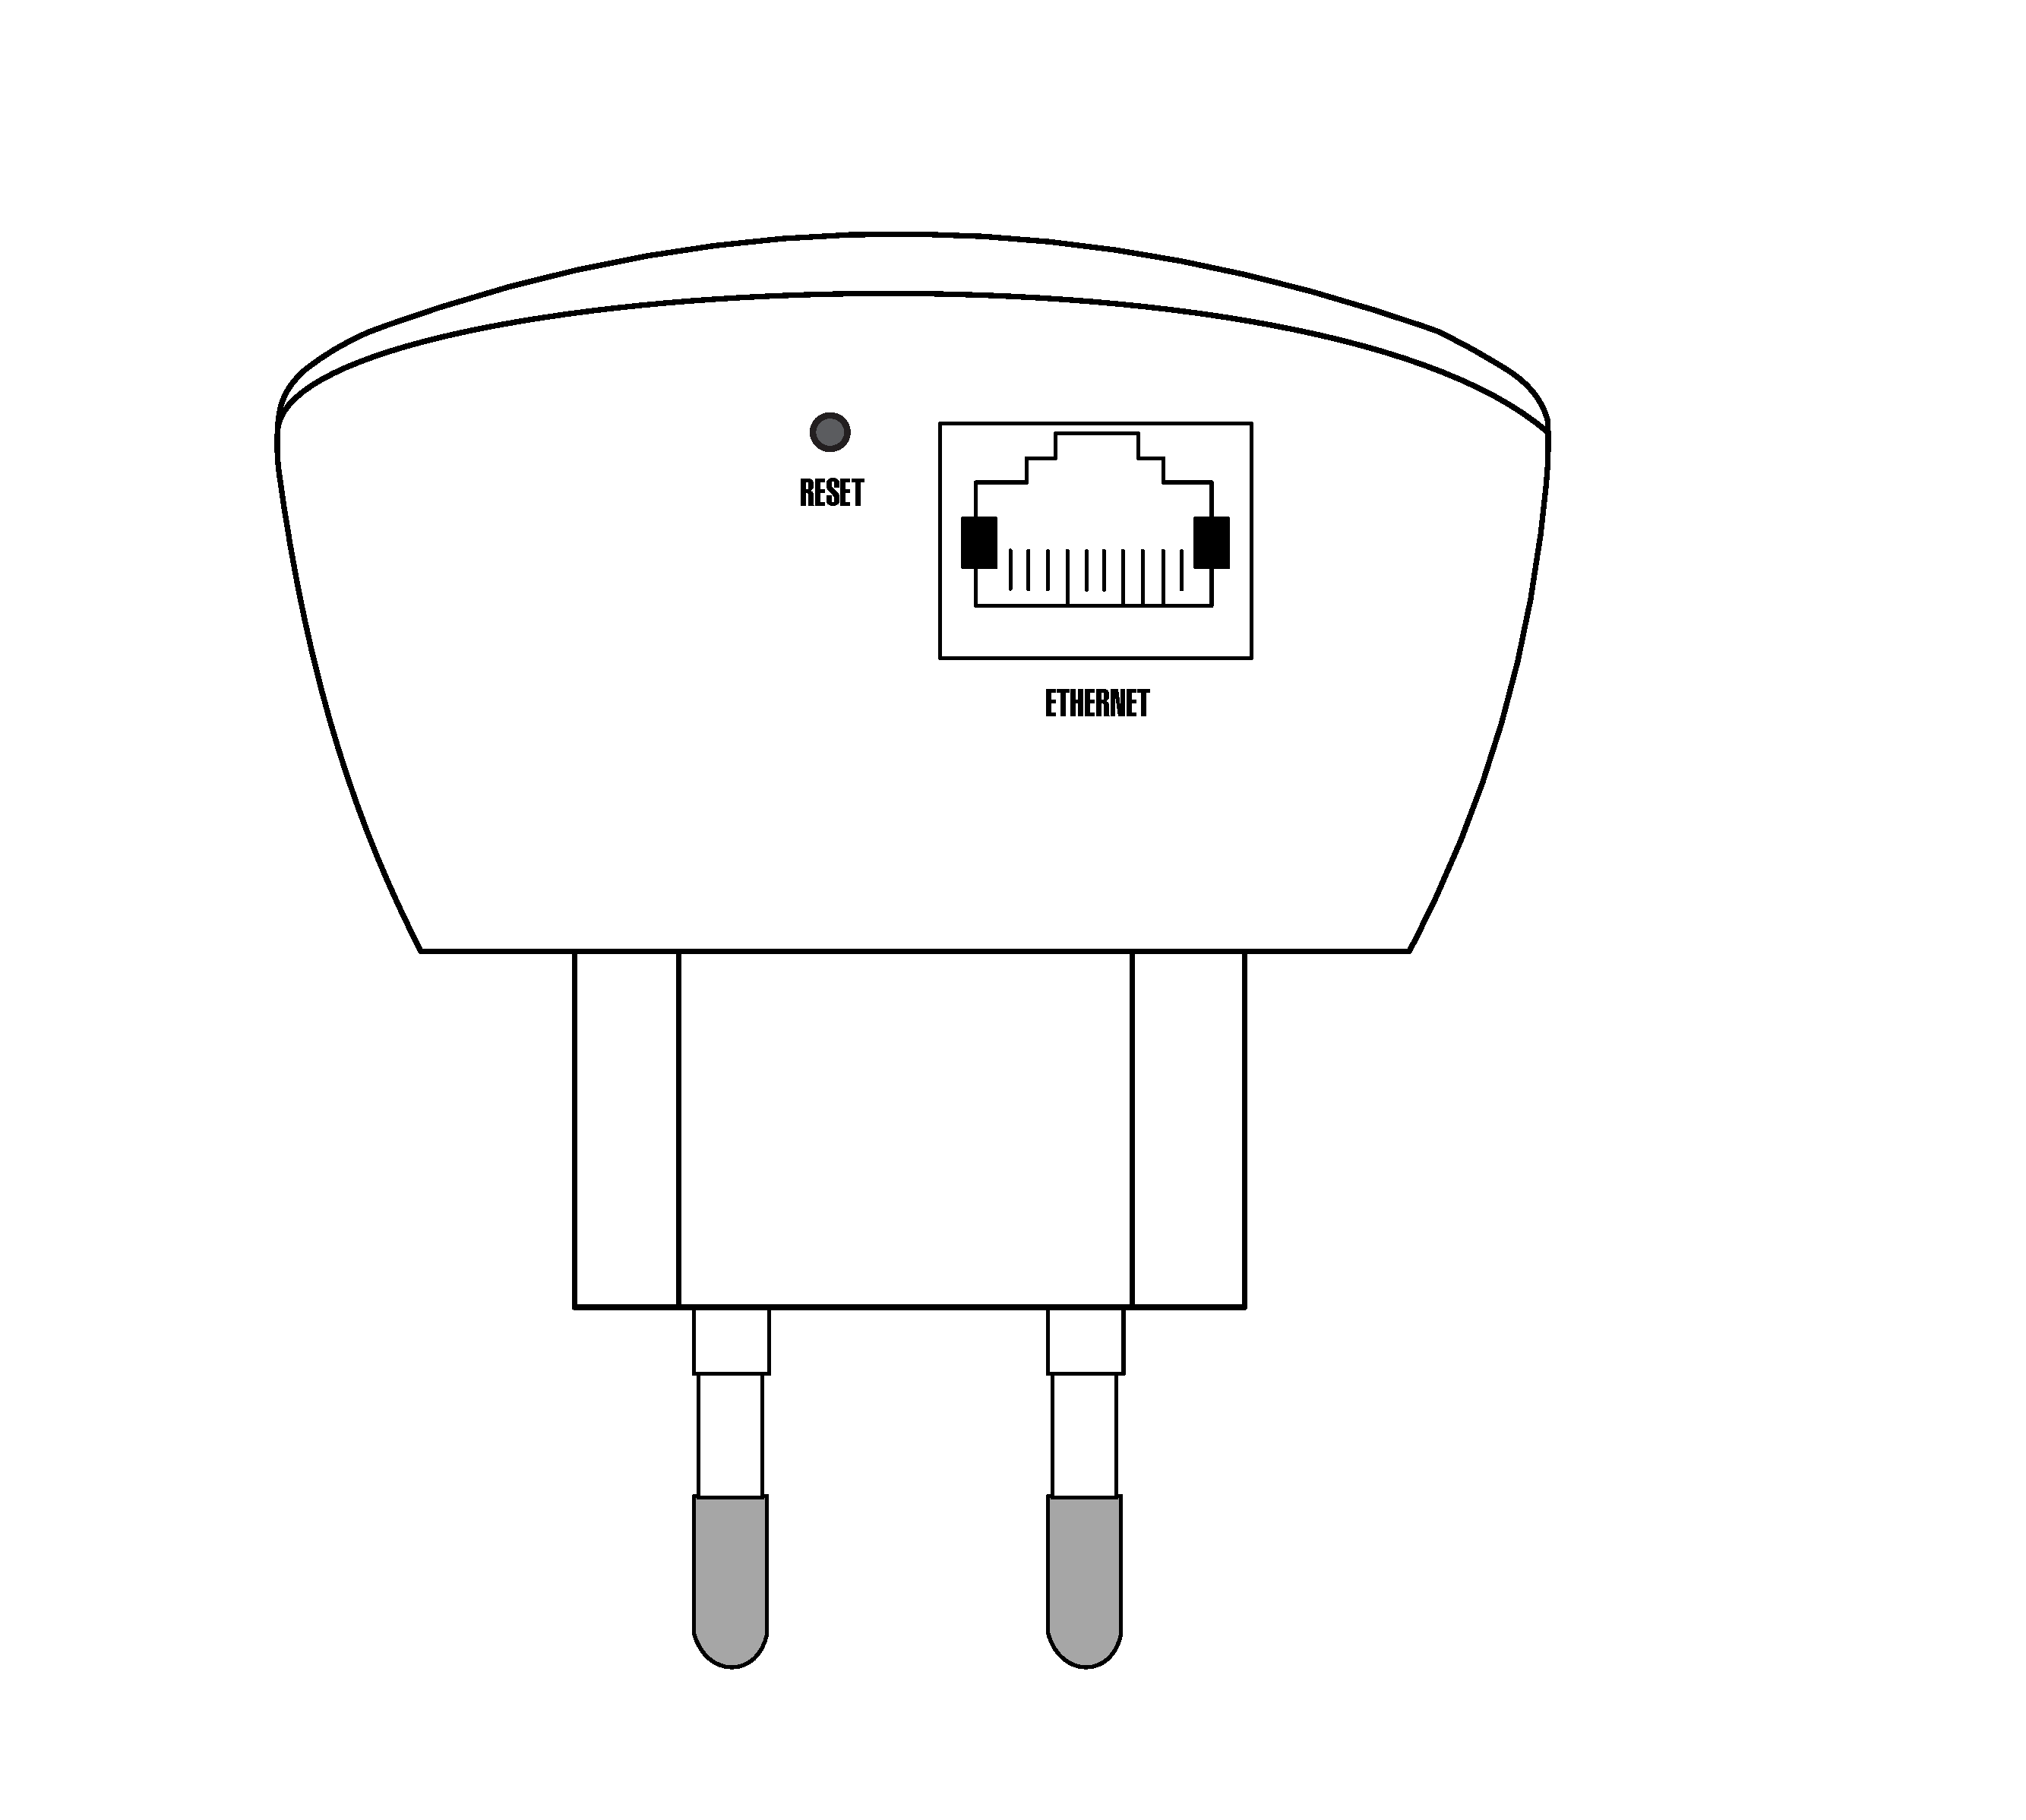
\includegraphics[%height=5cm, 
% 	width=0.5\textwidth]{./back.pdf}
% 	% 
\includegraphics[scale=0.25]{./site/\FFCommunity/logo.jpg}
% 	% }
%  % \caption{text} 
% % \end{figure} 
% % \def\rulecolor{\color{FFmagenta}}
% \textcolor{FFmagenta}{\rule{0.5\textwidth}{0.75mm}}
% {\columnbreak}\\
% \vspace{-1cm}
% \textcolor{FFmagenta}{\rule[1cm]{0.5\textwidth}{0.75mm}}

% dsfnbdsjfdsjf \\
% dsfndsfndsm,fn \\
% \end{multicols}

% \begin{multicols}{3}[{{\small und weiter mit drei Spalten}}]

% Hieran lässt sich die prinzipielle Funktionsweise von \LaTeX\,zeigen. Befehle werden immer mit einem führenden Backslash $\backslash$ in den bestehenden Text eingefügt. In der Präambel werden, wie bereits erwähnt, die für das gesamte Dokument gültigen Eigenschaften definiert. In obigem Beispiel wird zunächst festgelegt, um was für eine Art Dokument es sich handelt. Neben der Klasse "`article"' gibt es zahlreiche andere Klassen, die bereits standardmäßig zu \LaTeX\, gehören, wie "`report"', "`book"' oder "`letter"'. Andere, speziell an deutsche Bedürfnisse angepasste Klassen lassen sich entweder selbst erstellen oder aus dem Internet herunterladen. Mittels des Befehls \verb/\usepackage{german}/ wird \LaTeX\, angewiesen die deutsche Silbentrennung für das aktive Dokument anzuwenden. Zwischen \verb/\begin{document}/ und \verb/\end{document}/ steht der eigentliche Text. Hier lassen sich ebenfalls Befehle einbinden, die entweder die Struktur, oder die Formatierung einzelner Worte festlegen. Mittels section wird eine neue Gliederungsebene geöffnet, deren Überschrift "`Hier ist der Titel"' lautet. Mit einem einfachen Befehl lässt sich später automatisch ein vollständiges Inhaltsverzeichnis anlegen, was bei traditionellen Textverarbeitungen erfahrungsgemäß immer mit Problemen verbunden ist. Mit Hilfe spezieller Klassen lassen sich von juristischen Gutachten bis hin zu den eigenen Memoiren verschiedenste Dokumente erstellen. Das \LaTeX\,-Format kann auf allen Computersystemen problemlos verwendet werden, ohne mit Kompatibilitätsproblemen kämpfen zu müssen. \info{r}{\LaTeX}{als hervorragende Alternative zu Office!} Da \LaTeX\, nicht auf die system\-eigenen Schriften zurückgreift, sondern eigene mitbringt, besteht bei der Bearbeitung auf mehreren Systemen auch nicht das beispielsweise von Word bekannte Problem, dass Schriften willkürlich und ohne Warnung ersetzt werden. Was auf den ersten Blick sehr verwirrend erscheinen mag, ist bei näherer Betrachtung also sehr strukturiert und nachvollziehbar.
% \end{multicols} 

% |l|

% \begin{multicols}{3}{|l|l|}[\section*{Den Router Anschließen}]
% \vspace{-1cm}
% \textcolor{FFmagenta}{\rule[1cm]{0.5\textwidth}{0.75mm}}
% % \begin{figure}[h]
% % \makebox[width=0.5\textwidth]{ 
% 	% 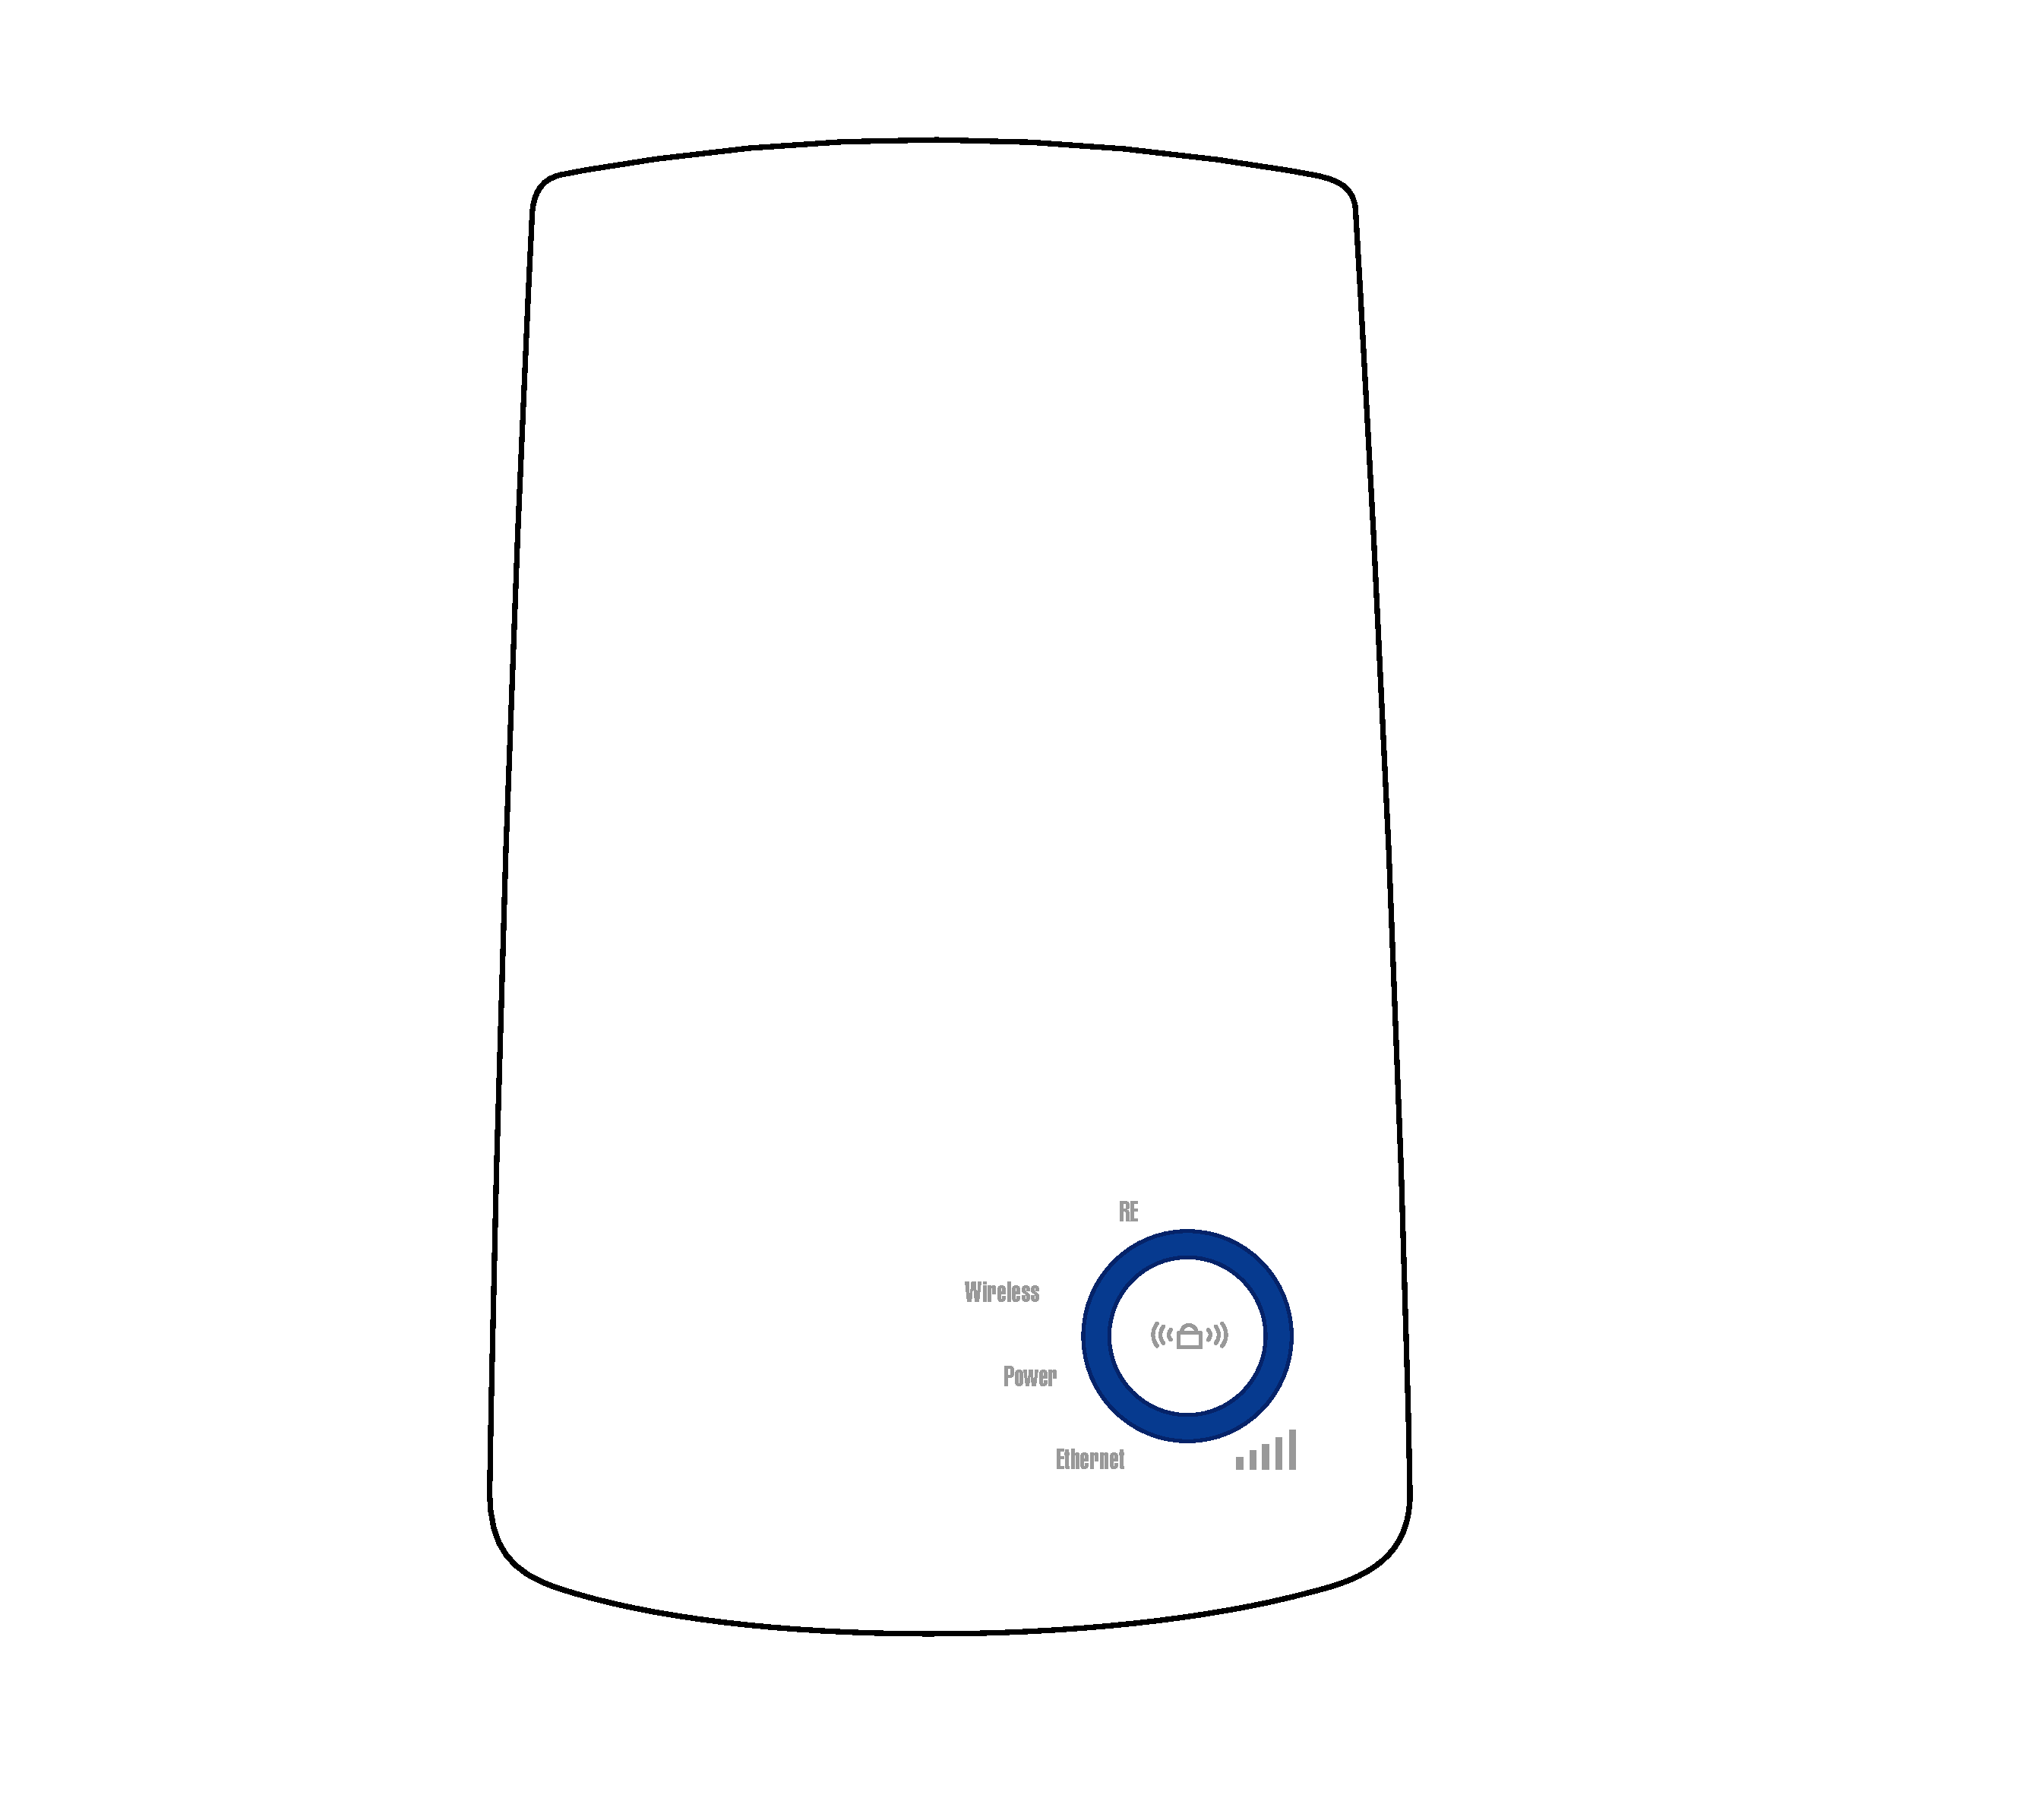
\includegraphics[scale=0.25]{./front.pdf}
% 	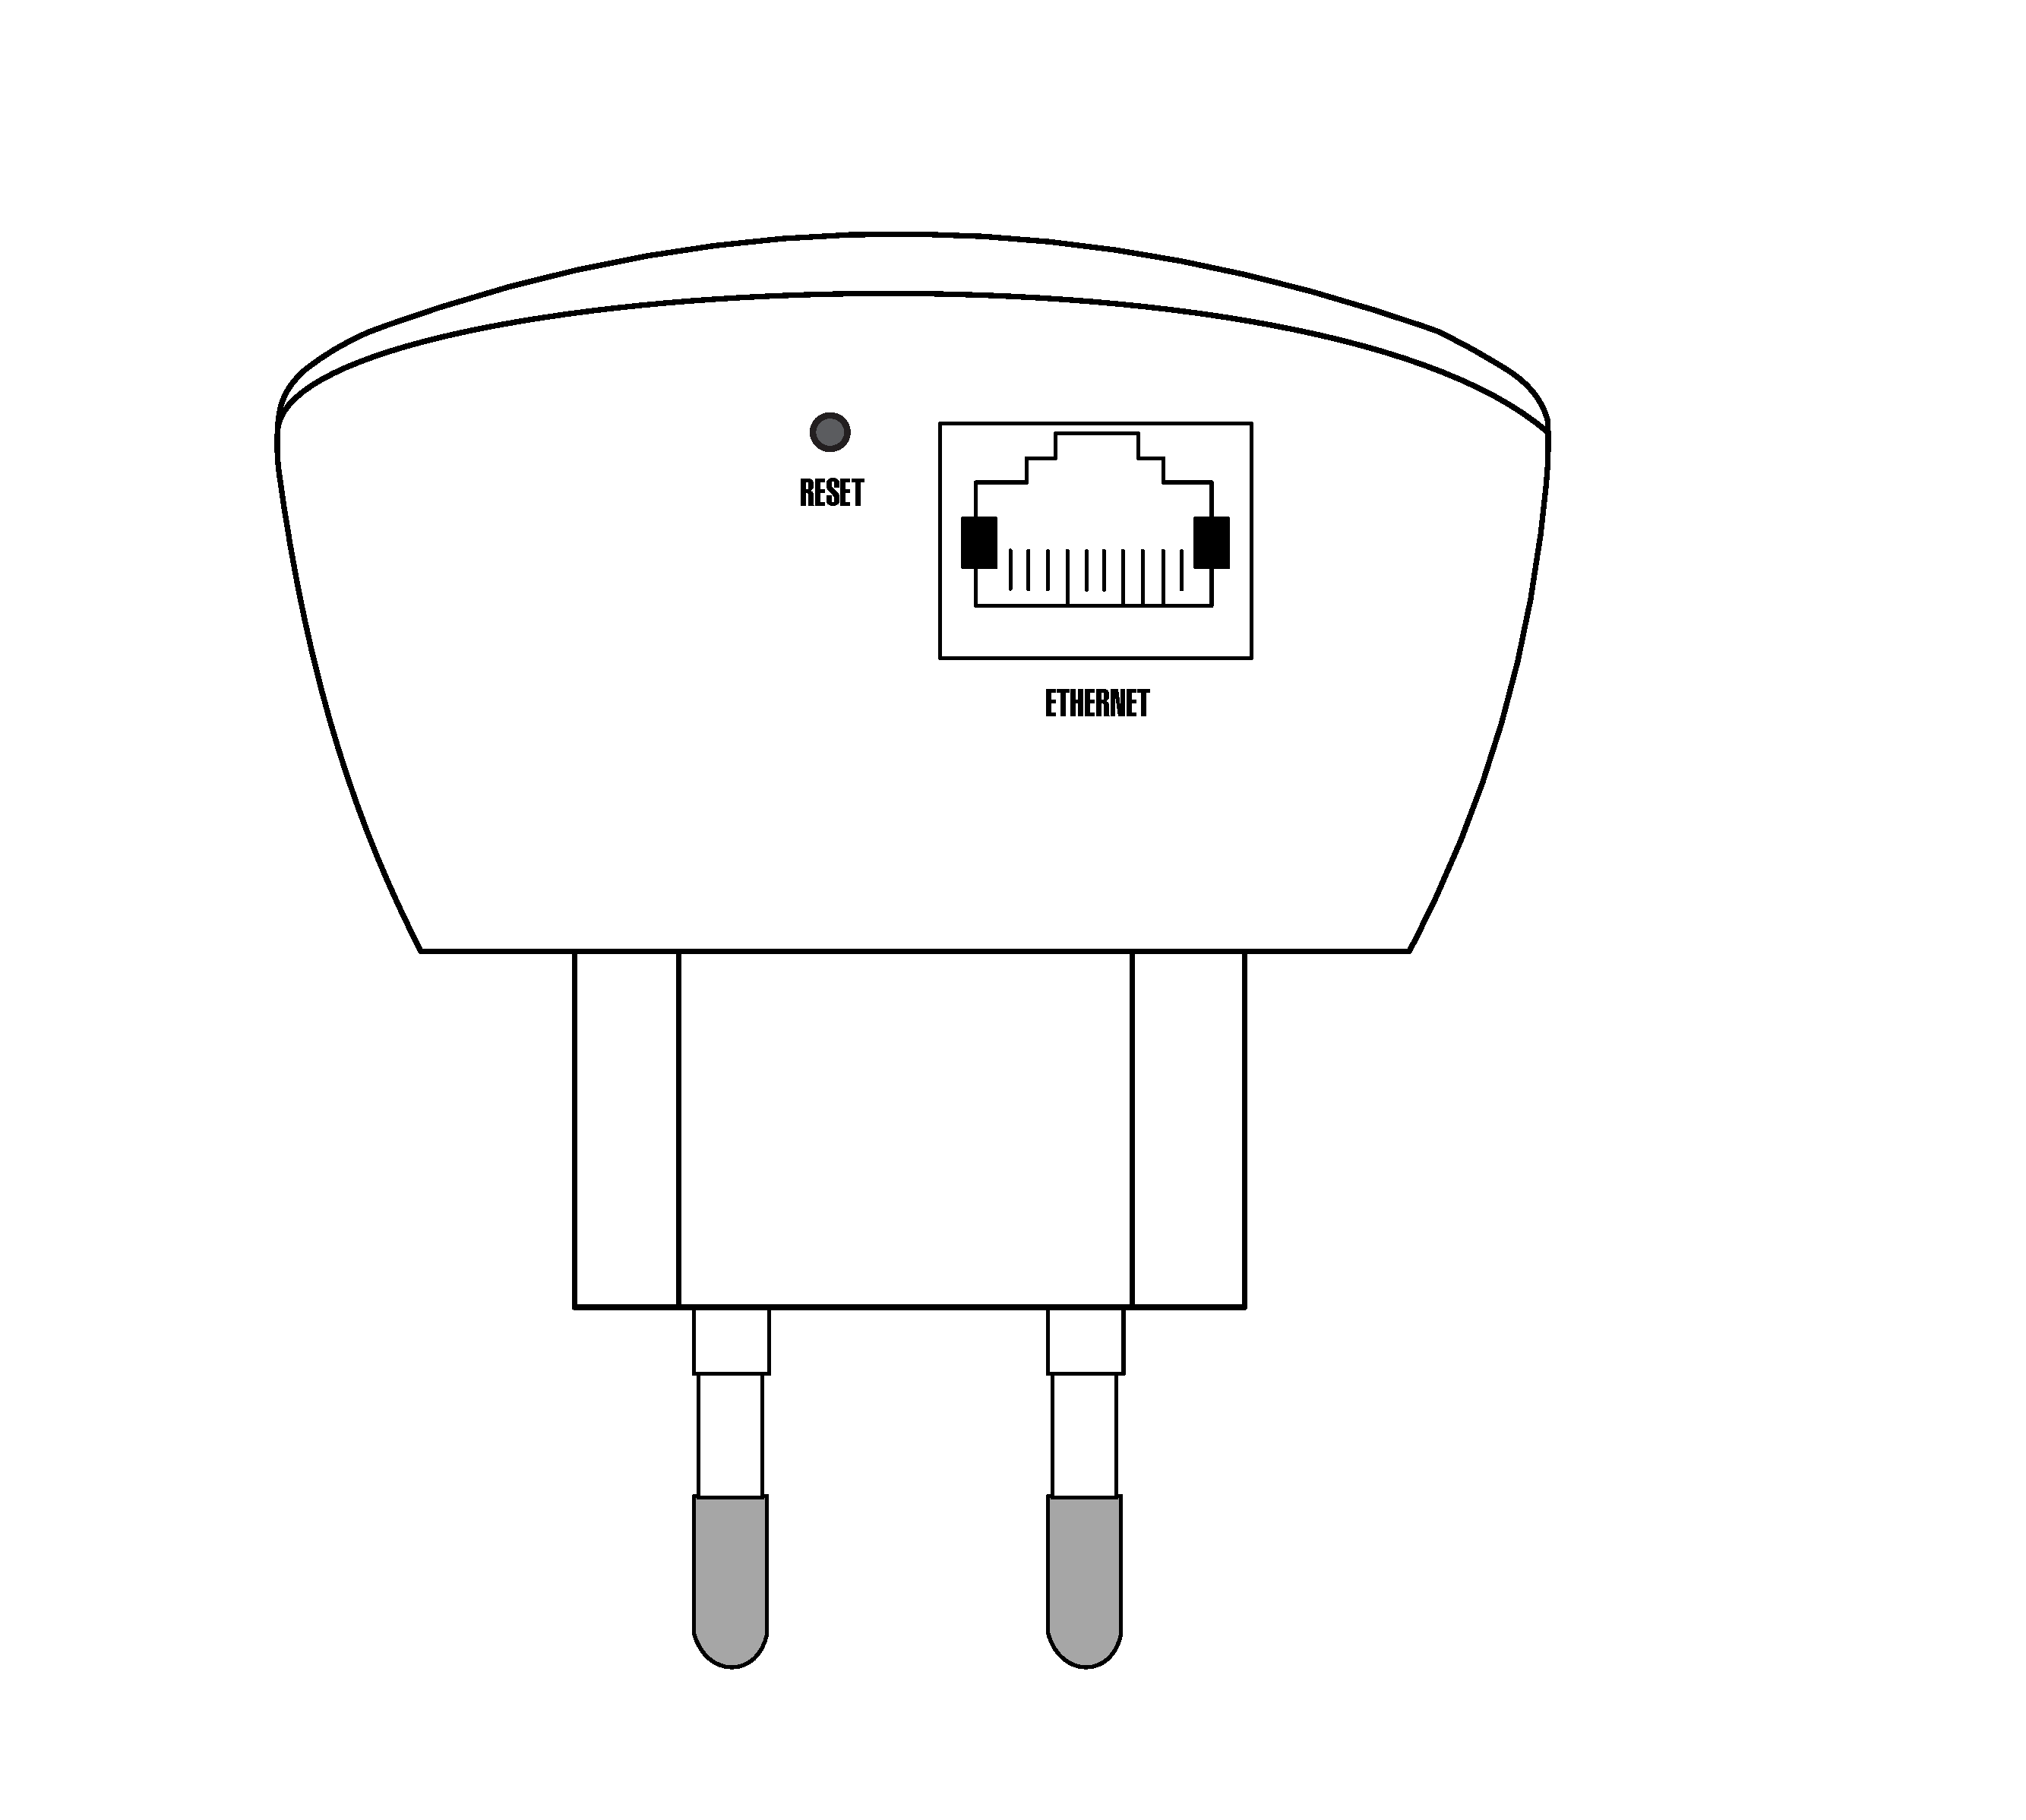
\includegraphics[%height=5cm, 
% 	width=0.5\textwidth]{./back.pdf}
% 	% 
\includegraphics[scale=0.25]{./site/\FFCommunity/logo.jpg}
% 	% }
%  % \caption{text} 
% % \end{figure} 
% % \def\rulecolor{\color{FFmagenta}}
% \textcolor{FFmagenta}{\rule{0.5\textwidth}{0.75mm}}
% {\columnbreak}\\
% \vspace{-1cm}
% \textcolor{FFmagenta}{\rule[1cm]{0.5\textwidth}{0.75mm}}

% dsfnbdsjfdsjf \\
% dsfndsfndsm,fn \\
% \end{multicols}

% \newpage

{\Huge Router anschließen}

\begin{table}[\textwidth]
\centering
 \setlength{\arrayrulewidth}{3pt}
\arrayrulecolor{FFmagenta}
\caption*{\Huge __}
% \caption*{\Huge Den Router Anschließen}
\label{my-label}
% \begin{tabular}{|p{0.33\textwidth}|>{\columncolor{FFmagenta}[0pt]}p{0.6\textwidth}|}
\begin{tabular}{|m{0.33\textwidth}|m{0.6\textwidth}|}
\hline
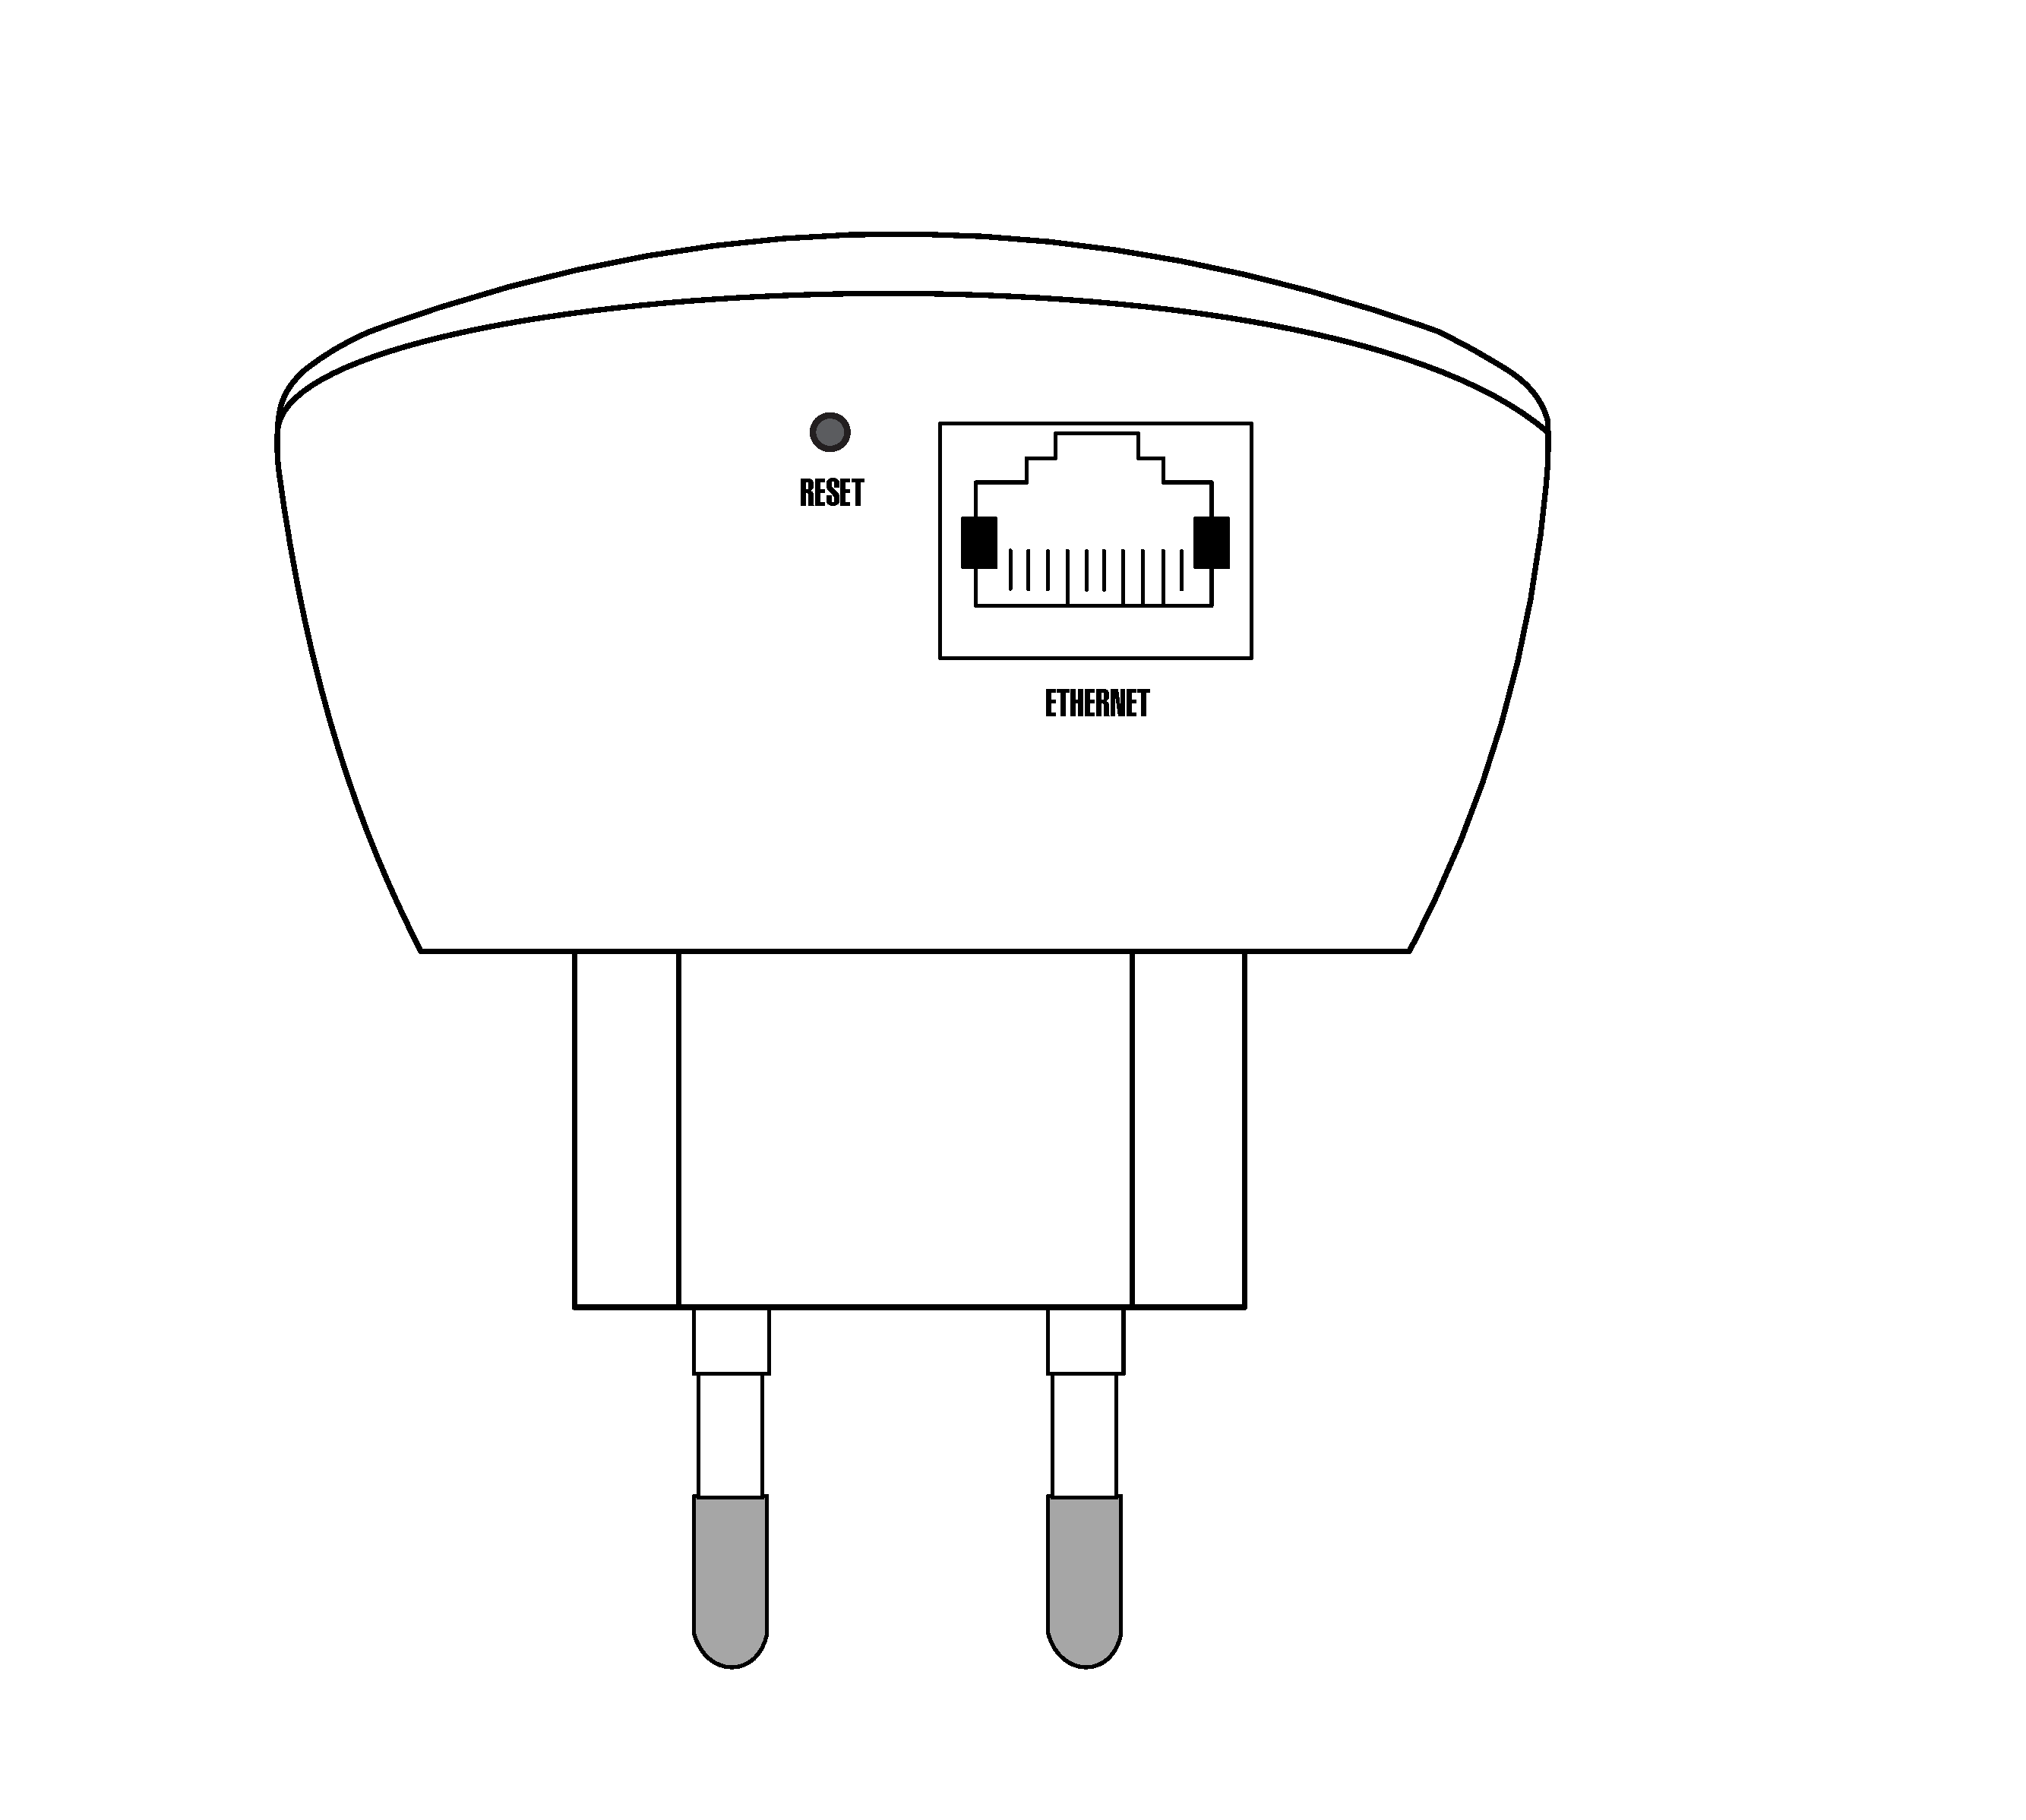
\includegraphics[%height=5cm, 
	width=0.33\textwidth]{./back.pdf} 
  %
  &
  % 
	\begin{minipage}{0.6\textwidth}
	Um die heruntergeladene Firmware installieren zu können, musst du deinen WLAN-Router mit deinem PC verbinden. \newline
  Schließe dazu als erstes den WLAN-Router mit dem Netzwerkkabel an eine Steckdose an. \newline

  Die Antennen, falls nicht Fest verbaut, kannst du jetzt oder auch später aufschrauben.
% \vspace{3.5cm}
\end{minipage}

\\
 % &  & \multicolumn{2}{l|}{} \\ \hline
 \hline
 % 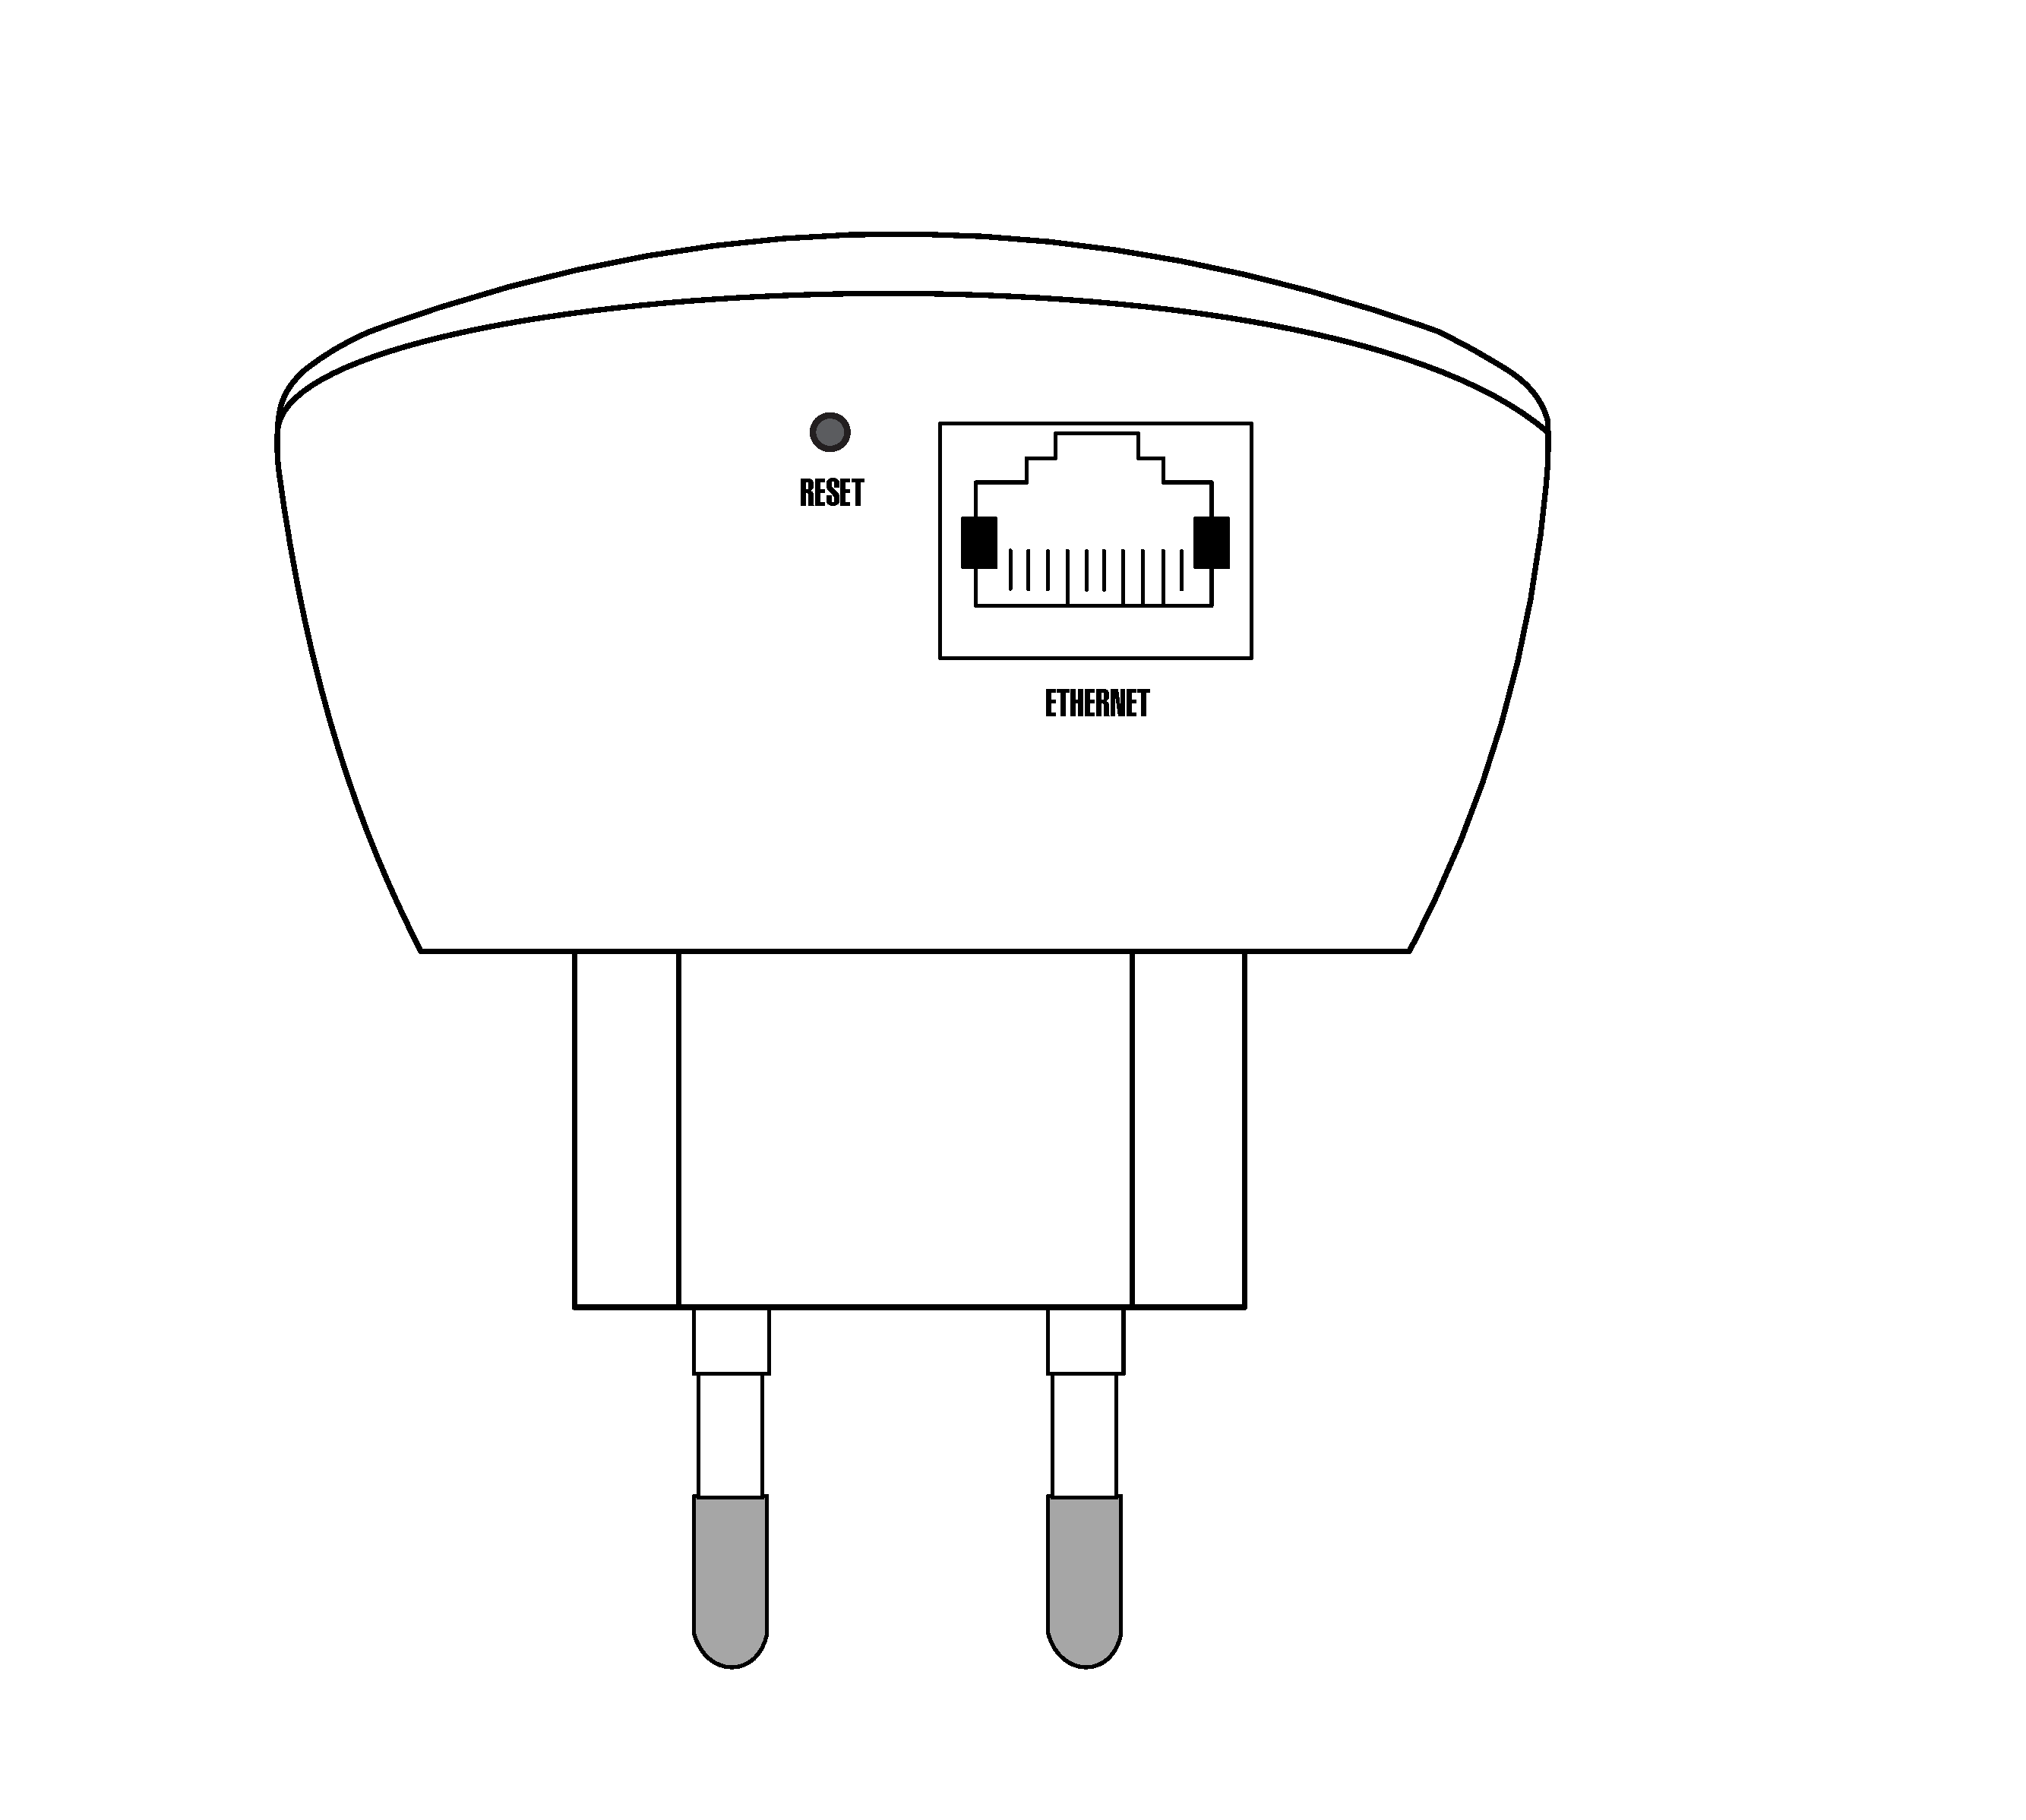
\includegraphics[%height=5cm, 
	% width=0.33\textwidth]{./back.pdf} & 
  %
  
	&
  %
	\begin{minipage}{0.6\textwidth}%
	\vspace{0.5cm}
  Verbinde den WLAN-Router anschließend mit Hilfe eines weiteren LAN-Kabels mit Deinem Computer. \newline
  Stecke dafür das Kabel in eine der gelben Buchsen (die blaue brauchst du später). \newline \newline

  Nach dem Einschalten braucht der WLAN-Router ungefähr 30 - 60 Sekunden, bevor er bereit ist. 
% \vspace{-1cm}
\end{minipage}

\\
 % &  & \multicolumn{2}{l|}{} \\ \hline
 \hline
\end{tabular}
\end{table}


\newpage

{\Huge Die Firmware installieren}



\begin{table}[\textwidth]
\centering
 \setlength{\arrayrulewidth}{3pt}
\arrayrulecolor{FFmagenta}
\caption*{\Huge __}
% \caption*{\Huge Den Router Anschließen}
\label{my-label}
% \begin{tabular}{|p{0.33\textwidth}|>{\columncolor{FFmagenta}[0pt]}p{0.6\textwidth}|}
\begin{tabular}{|m{0.33\textwidth}|m{0.6\textwidth}|}
\hline
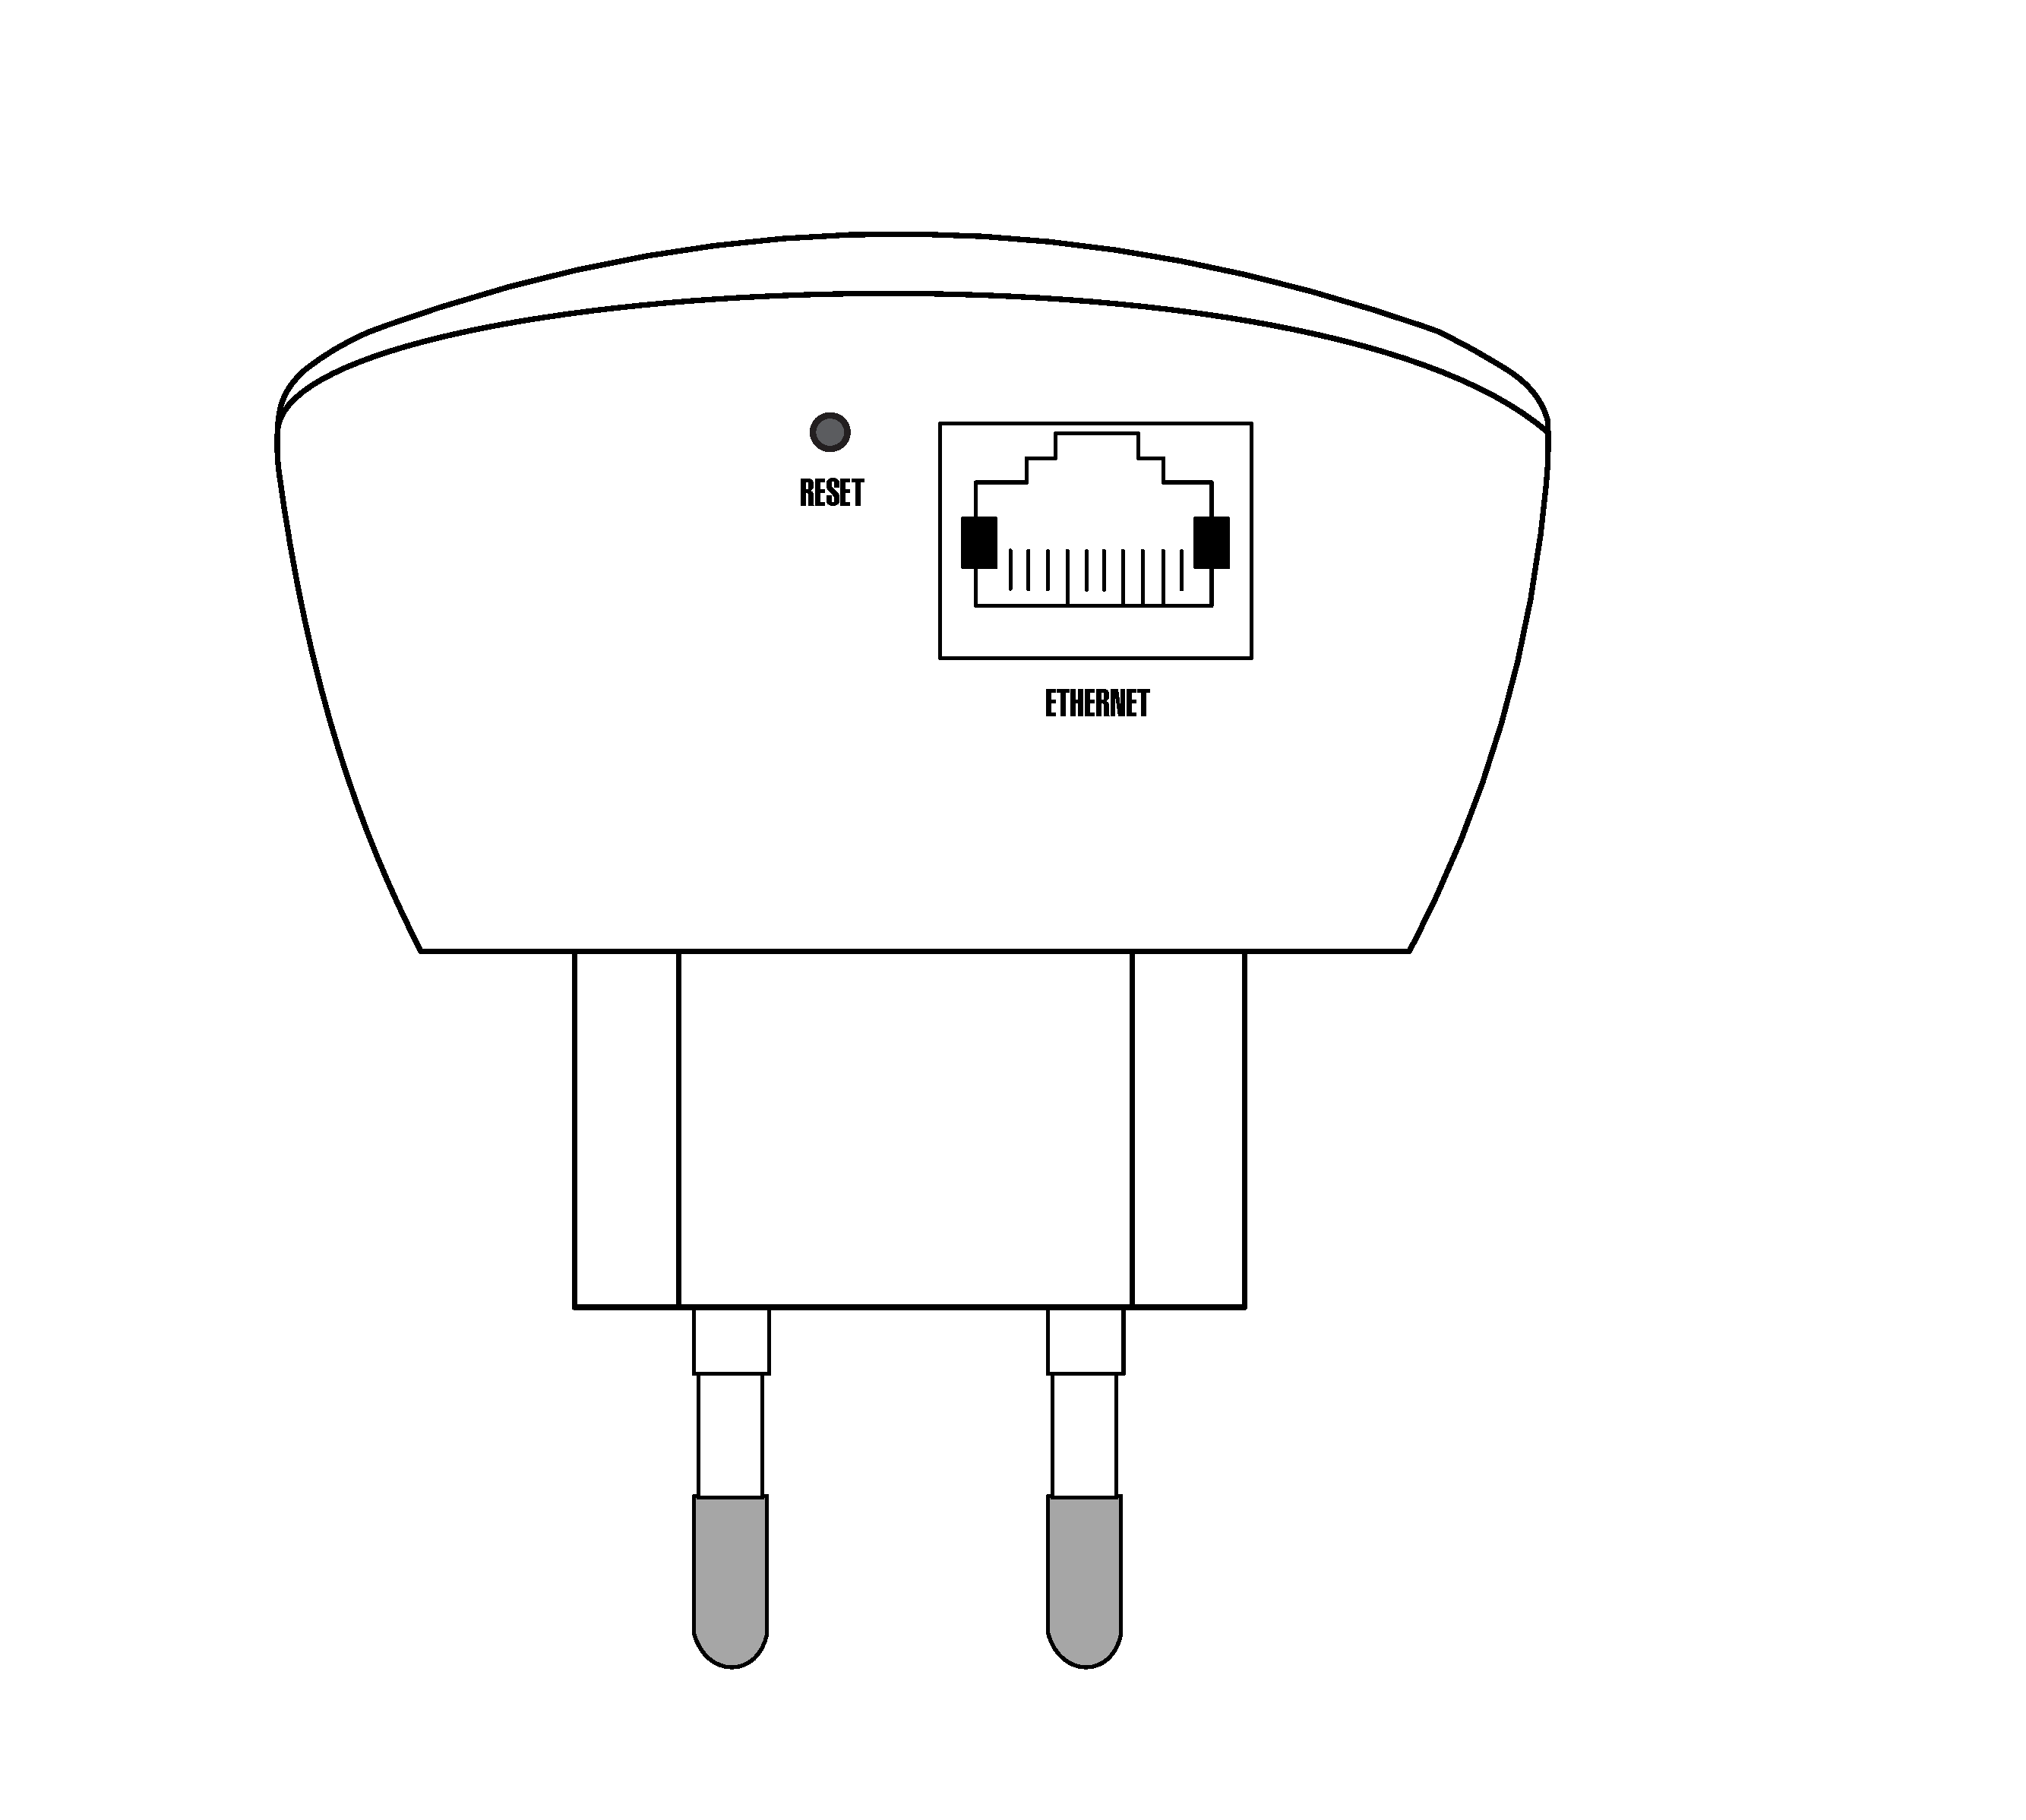
\includegraphics[%height=5cm, 
  width=0.33\textwidth]{./back.pdf} 
  %
  &
  % 
  \begin{minipage}{0.6\textwidth}
  Um die heruntergeladene Firmware installieren zu können, musst du deinen WLAN-Router mit deinem PC verbinden. \newline
  Schließe dazu als erstes den WLAN-Router mit dem Netzwerkkabel an eine Steckdose an. \newline

  Die Antennen, falls nicht Fest verbaut, kannst du jetzt oder auch später aufschrauben.
% \vspace{3.5cm}
\end{minipage}

\\
 % &  & \multicolumn{2}{l|}{} \\ \hline
 \hline
 % 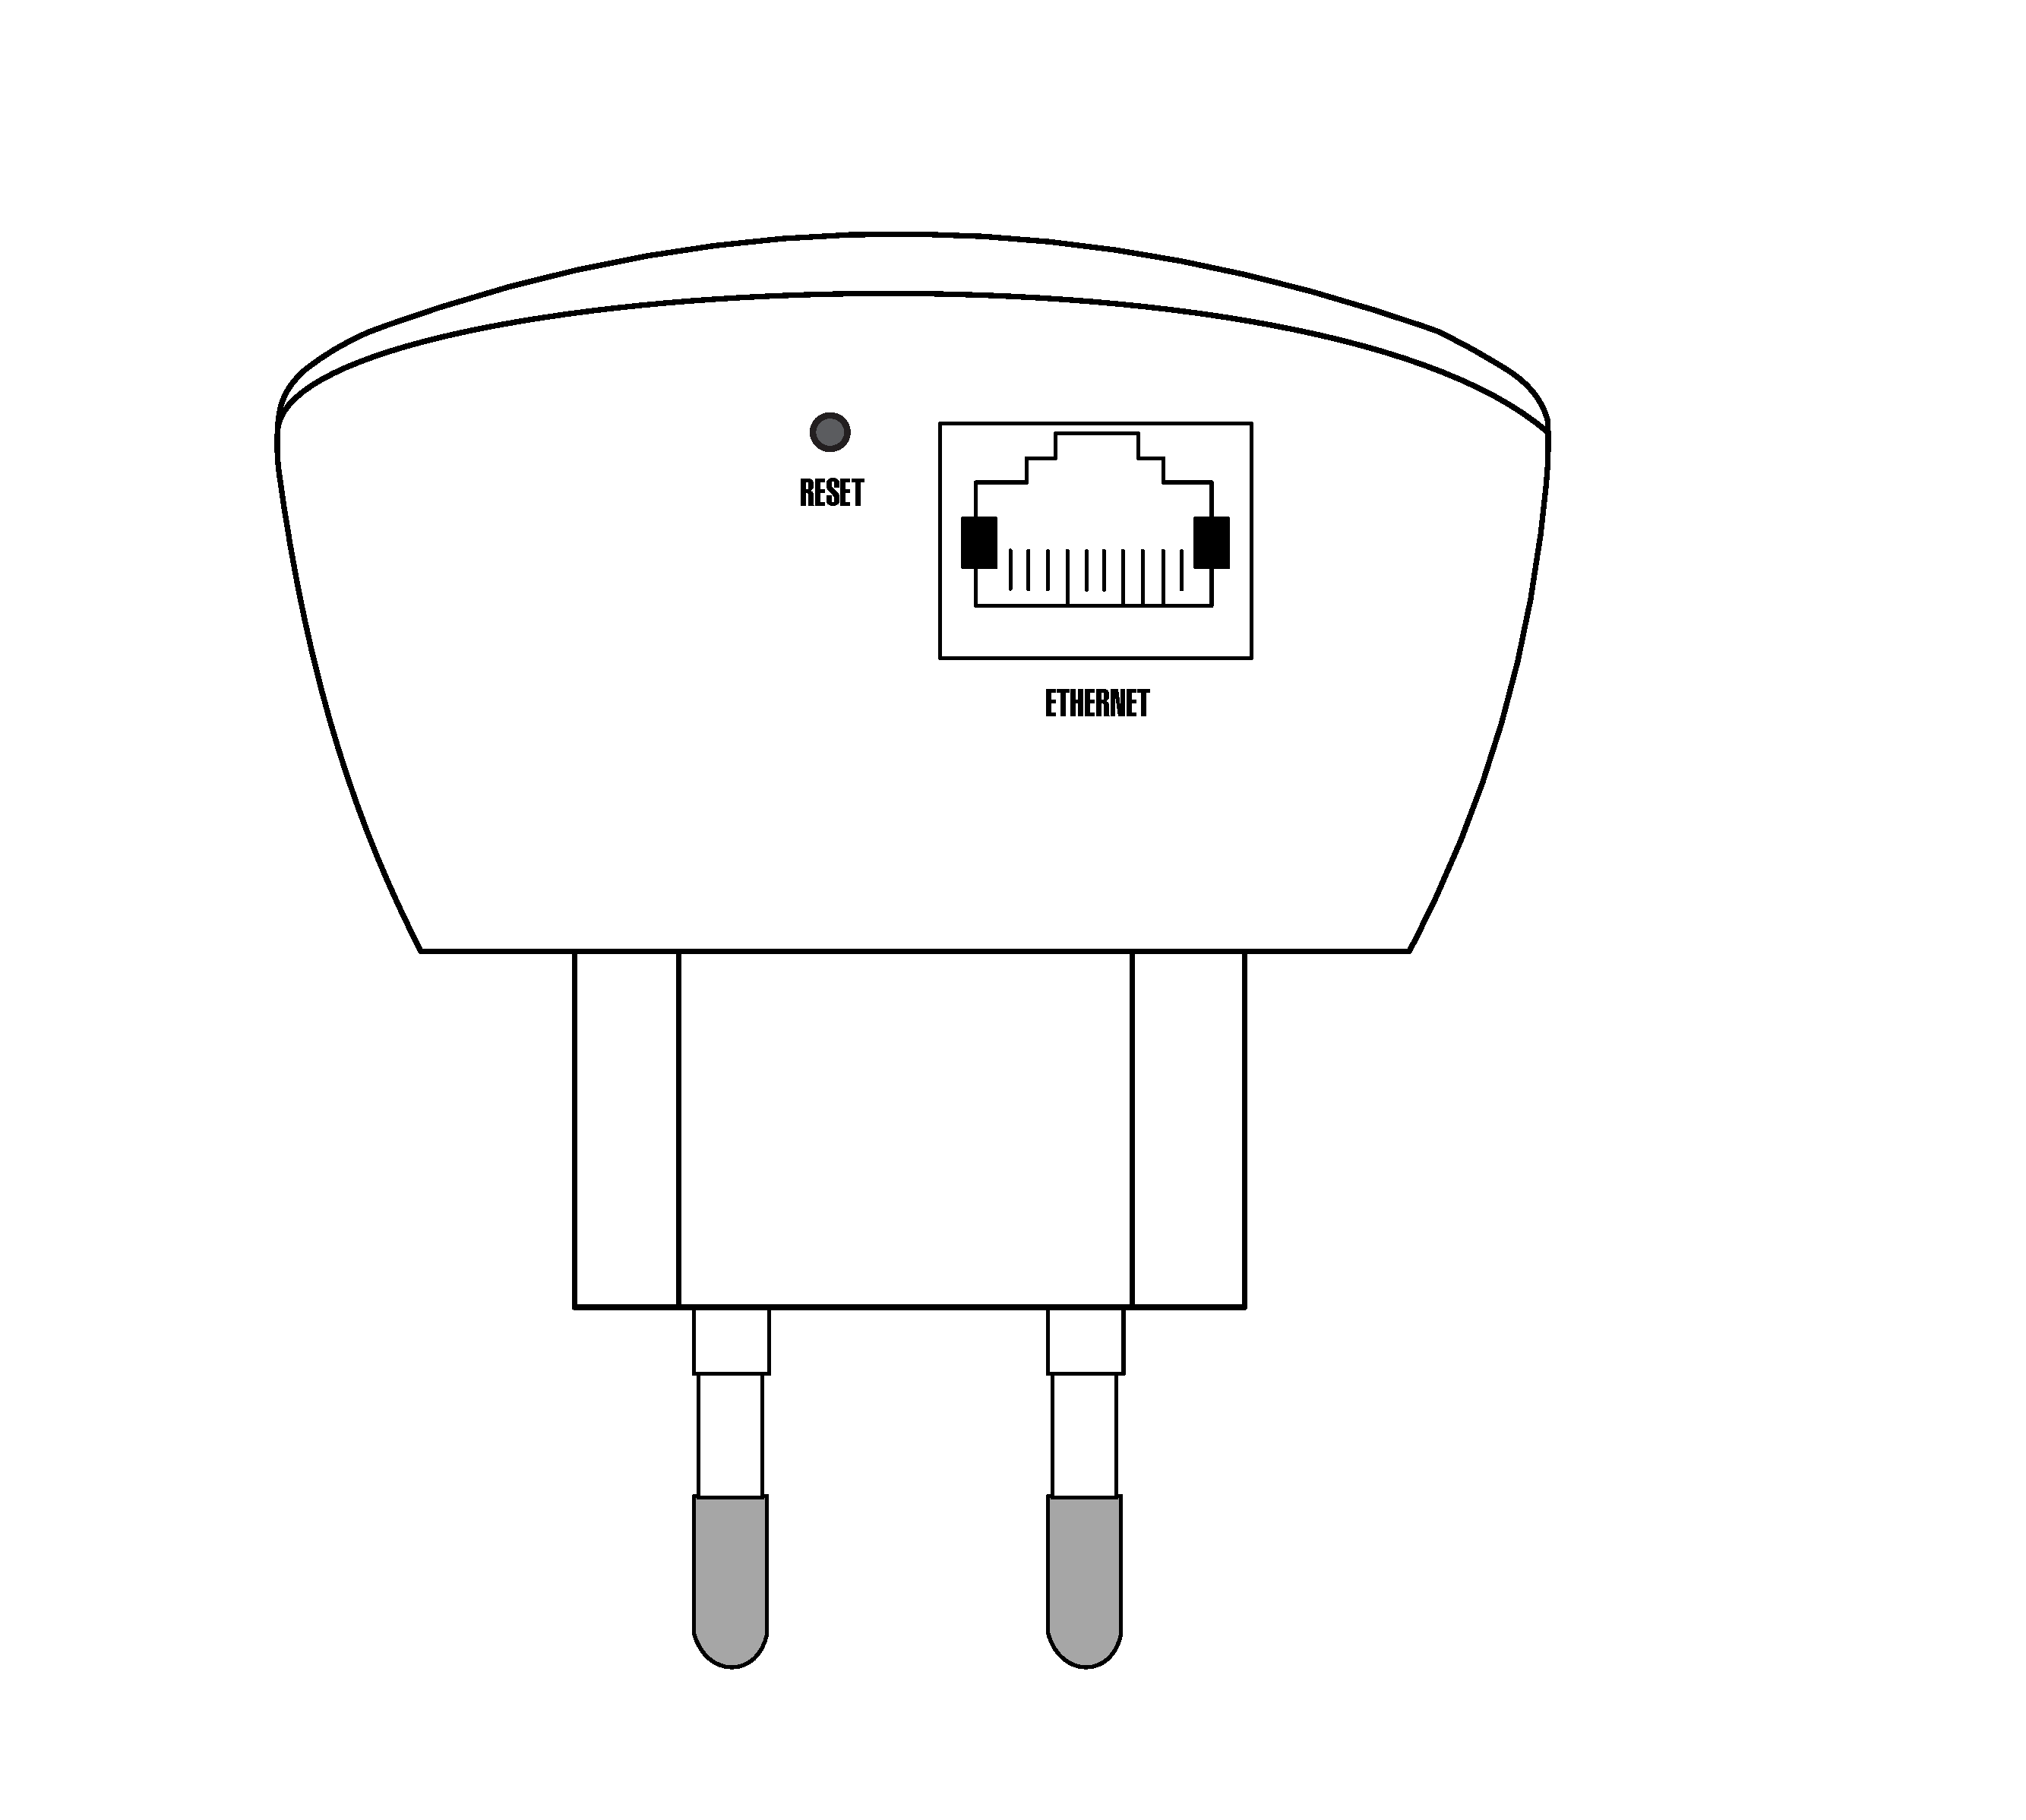
\includegraphics[%height=5cm, 
  % width=0.33\textwidth]{./back.pdf} & 
  %
  
  &
  %
  \begin{minipage}{0.6\textwidth}%
  \vspace{0.5cm}
  Verbinde den WLAN-Router anschließend mit Hilfe eines weiteren LAN-Kabels mit Deinem Computer. \newline
  Stecke dafür das Kabel in eine der gelben Buchsen (die blaue brauchst du später). \newline \newline

  Nach dem Einschalten braucht der WLAN-Router ungefähr 30 - 60 Sekunden, bevor er bereit ist. 
% \vspace{-1cm}
\end{minipage}

\\
 % &  & \multicolumn{2}{l|}{} \\ \hline
 \hline
\end{tabular}
\end{table}

%  sdhgbadskfhjasdk    Bild router




{\Large 3. Firmware einspielen} \\

Jetzt kannst du den Router einfach über den Webbrowser (z.B. Firefox) konfigurieren.\\ 
Dazu rufst du in die folgende Adresse auf: \\

% 2 Parameter 1. Die IP 2. die Farbe (für Freifunk: FFmagenta FFgelb FFblau)
\adressleiste{\stockip}{FFmagenta} \\

Der Menüpunkt \adressleiste{Systemtools}{FFgelb} erscheint nachdem man die Grundkonfiguration durchgeführt hat.

Du wirst anschließend zur Eingabe eines Benutzernamen und eines Passwortes gefragt. \\
Bei den Geräten von \printVendor gelten folgende Zugangsdaten:

\adressleiste{\printStockLogin}{FFblau} \\

% %  sdhgbadskfhjasdk    Bild router


% Anmelden am WLAN-Router (Benutzername und Passwort sind bei TP-Link Geräten jeweils admin)
% Nach der erfolgreichen Anmeldung müsste dein Browserfenster wie in folgender Abbildung aussehen. Klicke nun im Menü bitte auf den Eintrag “System Tools”.



% %  sdhgbadskfhjasdk    Bild router




% Als nächste wählst du aus dem Menü “Firmware Upgrade” (1). Danach kannst du die vorhin (in Schritt 2) heruntergeladene Datei auswählen (2). Nach einem Klick auf “Upgrade” (3) beginnt der Prozess.



% %  sdhgbadskfhjasdk    Bild router


% Du musst noch einmal kurz bestätigen …



% %  sdhgbadskfhjasdk    Bild router


% … und die Installation läuft.
% Wichtig: Während die Installation läuft, zieh bitte auf keinen Fall den Stecker oder das Netzwerk-Kabel aus dem Router ab. Die Installation sollte in ungefähr einer Minute abgeschlossen sein.



% %  sdhgbadskfhjasdk    Bild router




% {\Large 4. Abschluss} \\

% Nachdem die Firmware fertig installiert ist, startet der WLAN-Router neu. Dies ist u.a. am Blinken der Lämpchen des WLAN-Router zu erkennen. Zuerst blinken alle Lämpchen kurz auf, danach gehen sie aus. Wenn danach das Lämpchen mit dem Zahnrad gemütlich vor sich hin blinkt, ist der WLAN-Router im Konfigurationsmodus angekommen.

% Der WLAN-Router ist jetzt nicht mehr unter der angegeben Adresse erreichbar und eine Fehlermeldung erscheint. Das ist gut so. Denn nun läuft nicht mehr die TP-Link Firmware sondern die Freifunk Firmware auf deinem Router.



% %  sdhgbadskfhjasdk    Bild router


% Als nächstes musst du deinen Router noch einrichten und im Freifunk Netz anmelden. Auch das ist ganz einfach. Eine detaillierte Beschreibung findest du in der Anleitung "Freifunk-Fulda Knoten konfigurieren".

